\chapter{Implémentation, Tests et Résultats}

\section{Authentification JWT, Refresh Token et sécurité réseau}

\begin{itemize}
    \item \textbf{JWT (\texttt{HS256}) et Refresh Token rotatif} : jeton d'accès valable 24\,h (\texttt{JwtTokenProvider.java}), associé à un \texttt{RefreshToken} de 7\,jours stocké haché en \textbf{SHA-256} (\texttt{/auth/refresh}, \texttt{/auth/logout}).
    \item \textbf{Protection anti-force brute} : verrouillage de 5\,minutes après 5 échecs de connexion et filtre \texttt{RateLimitingFilter} (20\,req/min/IP sur \texttt{/auth/login}, \texttt{/vote/request-otp}, \texttt{/vote/verify-otp}), avec résolution d'IP réelle derrière proxy (\texttt{ClientIpResolver}).
    \item \textbf{Réinitialisation} : \texttt{/auth/forgot-password} génère un code à 6 chiffres (validité 15\,min, hash BCrypt) et renvoie une réponse neutre anti-énumération ; \texttt{/auth/reset-password} met à jour le mot de passe et révoque les sessions actives.
\end{itemize}

\section{Vote sécurisé, chiffrement AES-256-GCM et chaînage SHA-256}

Le protocole de vote (\texttt{VotingService.java}, L94--L228) s'exécute en trois étapes :
\begin{enumerate}
    \item \textbf{Demande d'OTP (\texttt{/vote/request-otp})} : vérification de la fenêtre temporelle, de l'éligibilité, de l'unicité, du quota (5/h) et du cooldown (60\,s) ; génération d'un code 6 chiffres via \texttt{SecureRandom}, haché en \textbf{BCrypt} et envoyé par e-mail (Brevo HTTPS API en production, SMTP MailHog en local).
    \item \textbf{Vérification OTP (\texttt{/vote/verify-otp})} : maximum 5 tentatives (validité 5\,min) ; délivre un \texttt{VoteToken} SHA-256 à usage unique (validité 10\,min).
    \item \textbf{Dépôt du bulletin (\texttt{/vote/submit})} : transaction \texttt{@Transactional} chiffrant le choix en \textbf{AES-256-GCM} (IV aléatoire 12\,octets, clé dérivée par \textbf{PBKDF2WithHmacSHA256} sur 65\,536 itérations), calculant l'empreinte chaînée \textbf{SHA-256}, enregistrant l'émargement (\texttt{VoterAuditLog}) et invalidant le \texttt{VoteToken}.
\end{enumerate}

\begin{uaszbox}{Chaînage SHA-256 des bulletins (\texttt{Ballot} \& \texttt{AuditService})}
Chaque bulletin référence l'empreinte du bulletin précédent (\texttt{previousHash}, initialisée à \texttt{"GENESIS"}) et un numéro de séquence :
$$\text{ballotHash}_n = \text{SHA-256}\left(\text{previousHash}_n \,\|\, \text{encryptedPayload}_n \,\|\, \text{sequenceNumber}_n\right)$$
\texttt{AuditService.verifyBallotChain()} vérifie l'intégrité séquentielle de la chaîne. Lors de la validation locale sur le scrutin \textit{L3 Informatique 2026} (25 votes), \texttt{verifyBallotChain()} a retourné \texttt{chainValid = true}.
\end{uaszbox}

\section{Temps réel, PV PDF et réclamations}

\begin{itemize}
    \item \textbf{WebSocket STOMP} : diffusion des résultats sur \texttt{/topic/results/\{id\}} sécurisée par \texttt{ChannelInterceptor}, alimentant automatiquement les graphiques \textbf{Chart.js} côté Angular.
    \item \textbf{Procès-Verbal PDF} : génération programmatique via \textbf{OpenPDF 1.3.30} (\texttt{PdfReportService.java}) dès l'état \texttt{CLOTURE}.
    \item \textbf{Réclamations} : dépôt autorisé uniquement aux états \texttt{PUBLICATION} et \texttt{CLOTURE} dans un délai de 48\,heures après \texttt{dateFin} (\texttt{ComplaintService.java}).
\end{itemize}

\section{Interfaces applicatives réalisées}

Les captures ci-après ont été réalisées sur l'environnement local peuplé avec des données fictives réalistes de l'UASZ (desktop \texttt{1440x900} et mobile \texttt{390x844}).

\subsection{Authentification et réinitialisation}
Les figures~\ref{fig:login-desktop}, \ref{fig:login-mobile}, \ref{fig:forgot} et~\ref{fig:reset} illustrent la page de connexion compacte (desktop et mobile) ainsi que les modes de réinitialisation de mot de passe.

\begin{figure}[H]
    \centering
    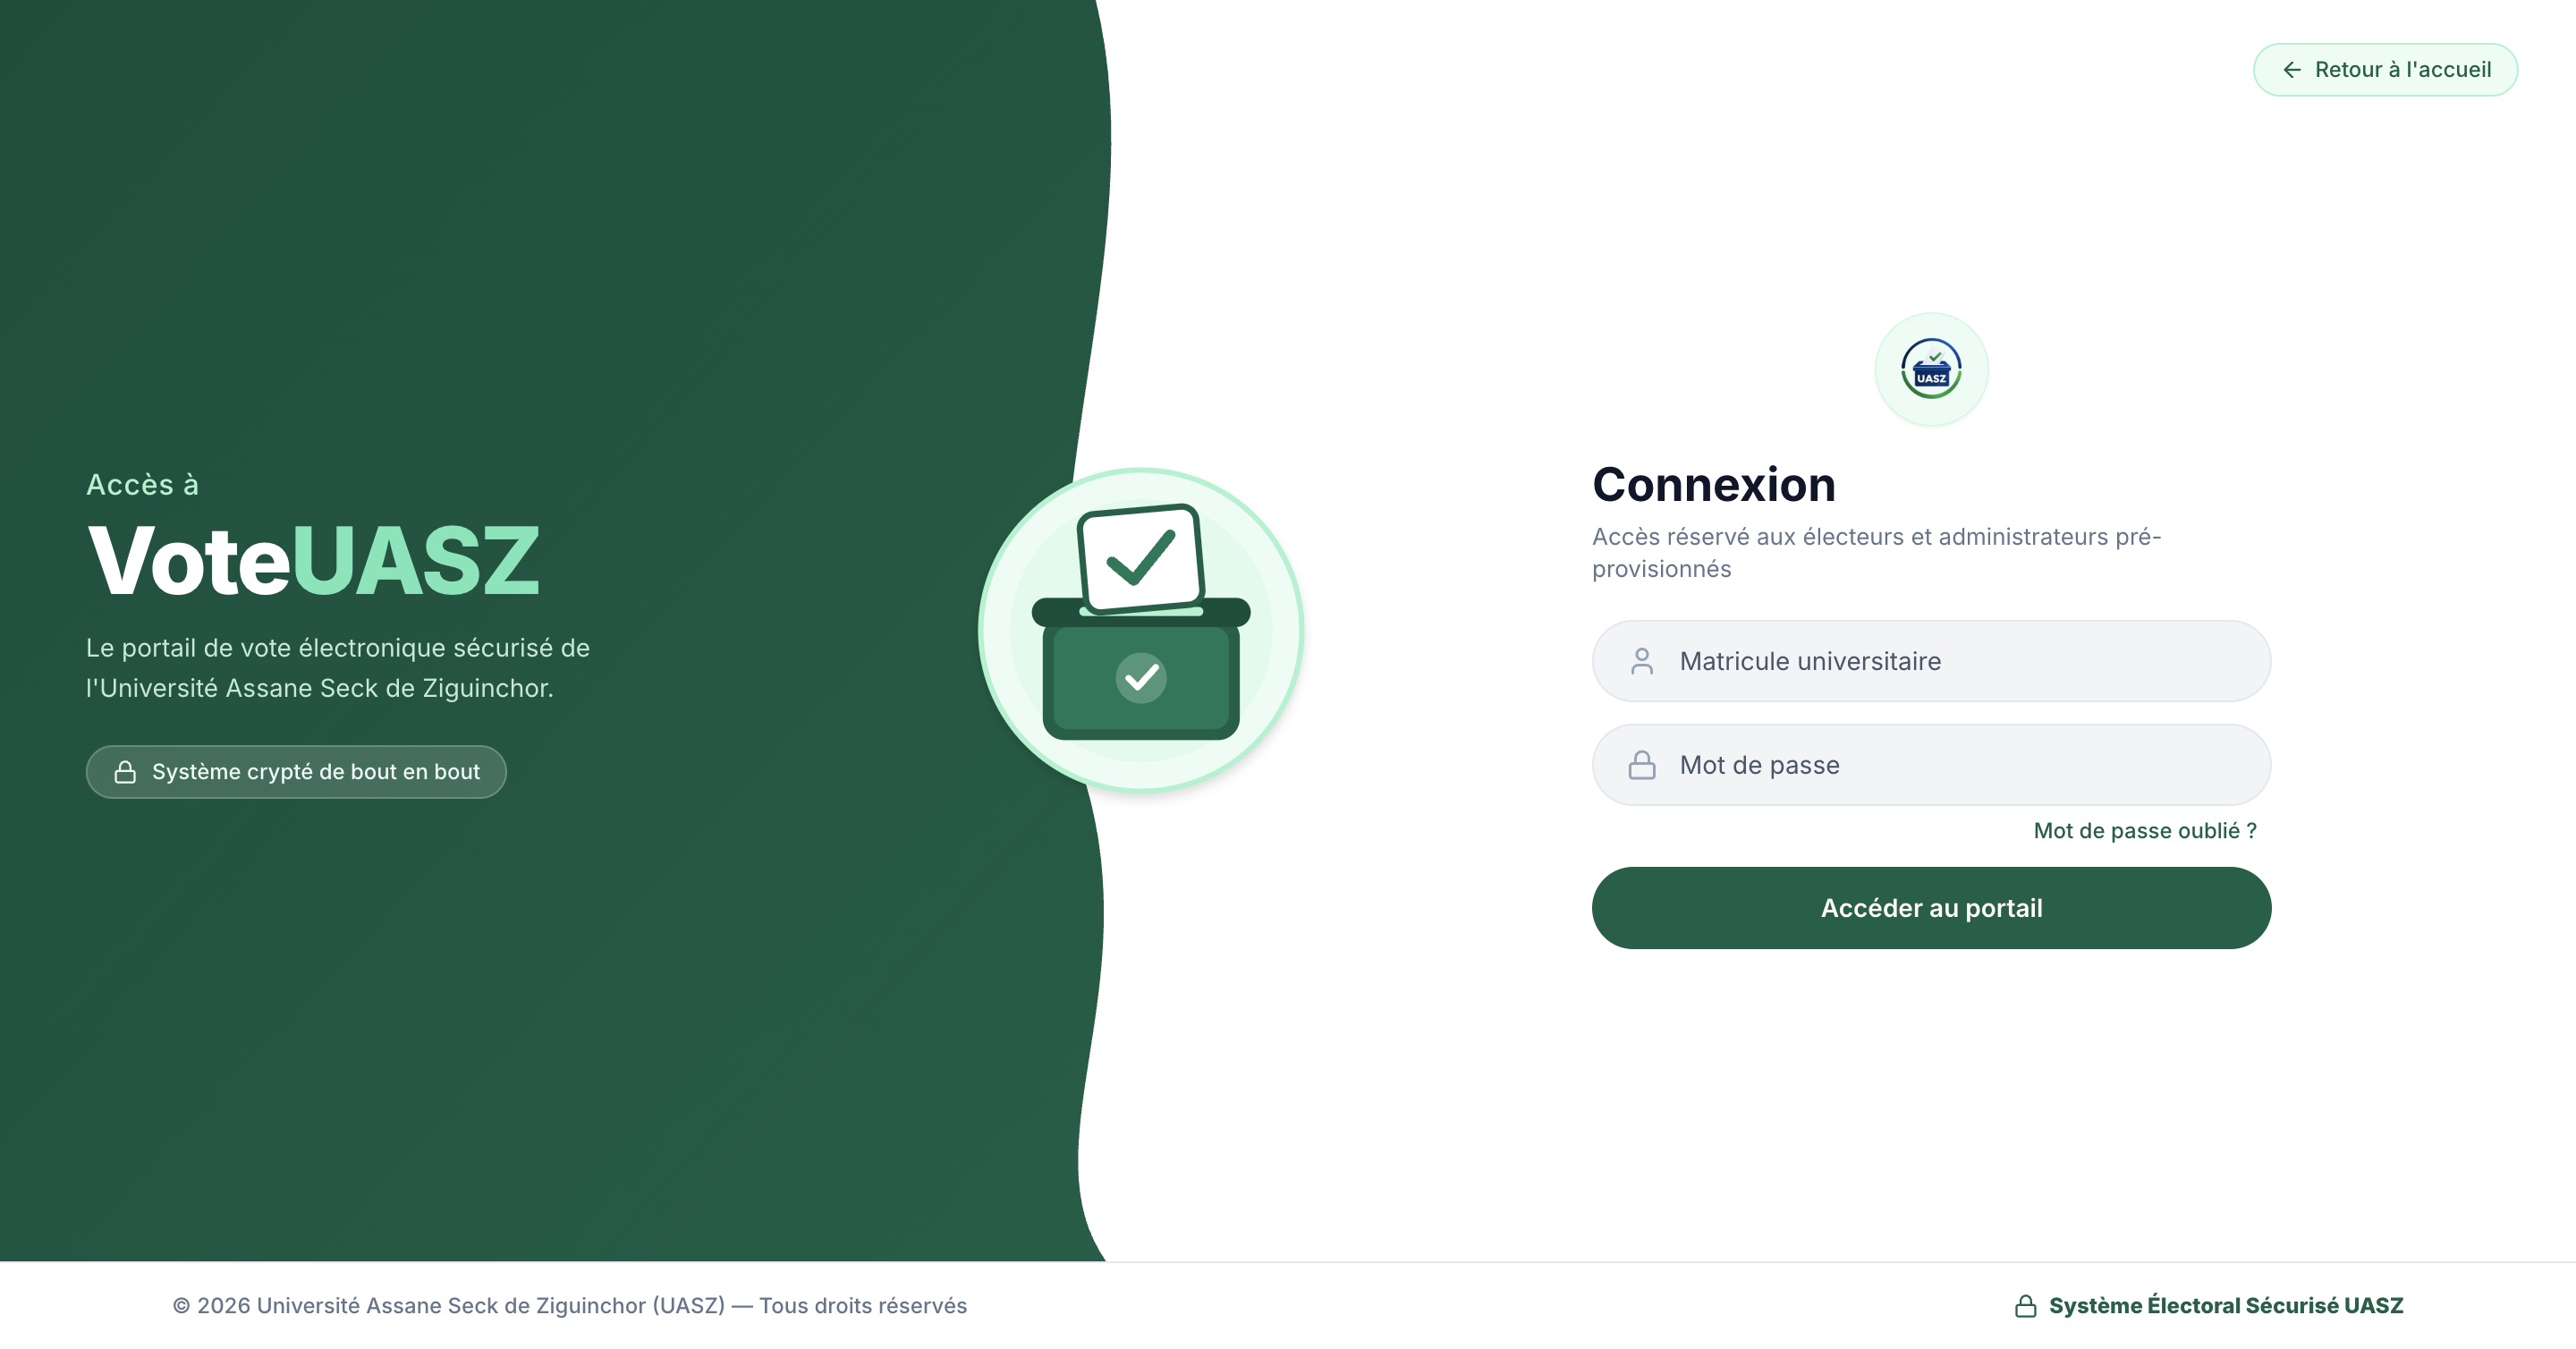
\includegraphics[width=0.88\textwidth,height=0.45\textheight,keepaspectratio]{3-2-1-login-desktop.png}
    \caption{Page de connexion compacte en mode desktop (\texttt{1440x900})}
    \label{fig:login-desktop}
\end{figure}

\begin{figure}[H]
    \centering
    \begin{minipage}{0.38\textwidth}
        \centering
        
\includegraphics[width=\textwidth,height=0.42\textheight,keepaspectratio]{3-2-1-login-mobile.png}
        \caption{Connexion mobile (\texttt{390x844})}
        \label{fig:login-mobile}
    \end{minipage}
    \hfill
    \begin{minipage}{0.58\textwidth}
        \centering
        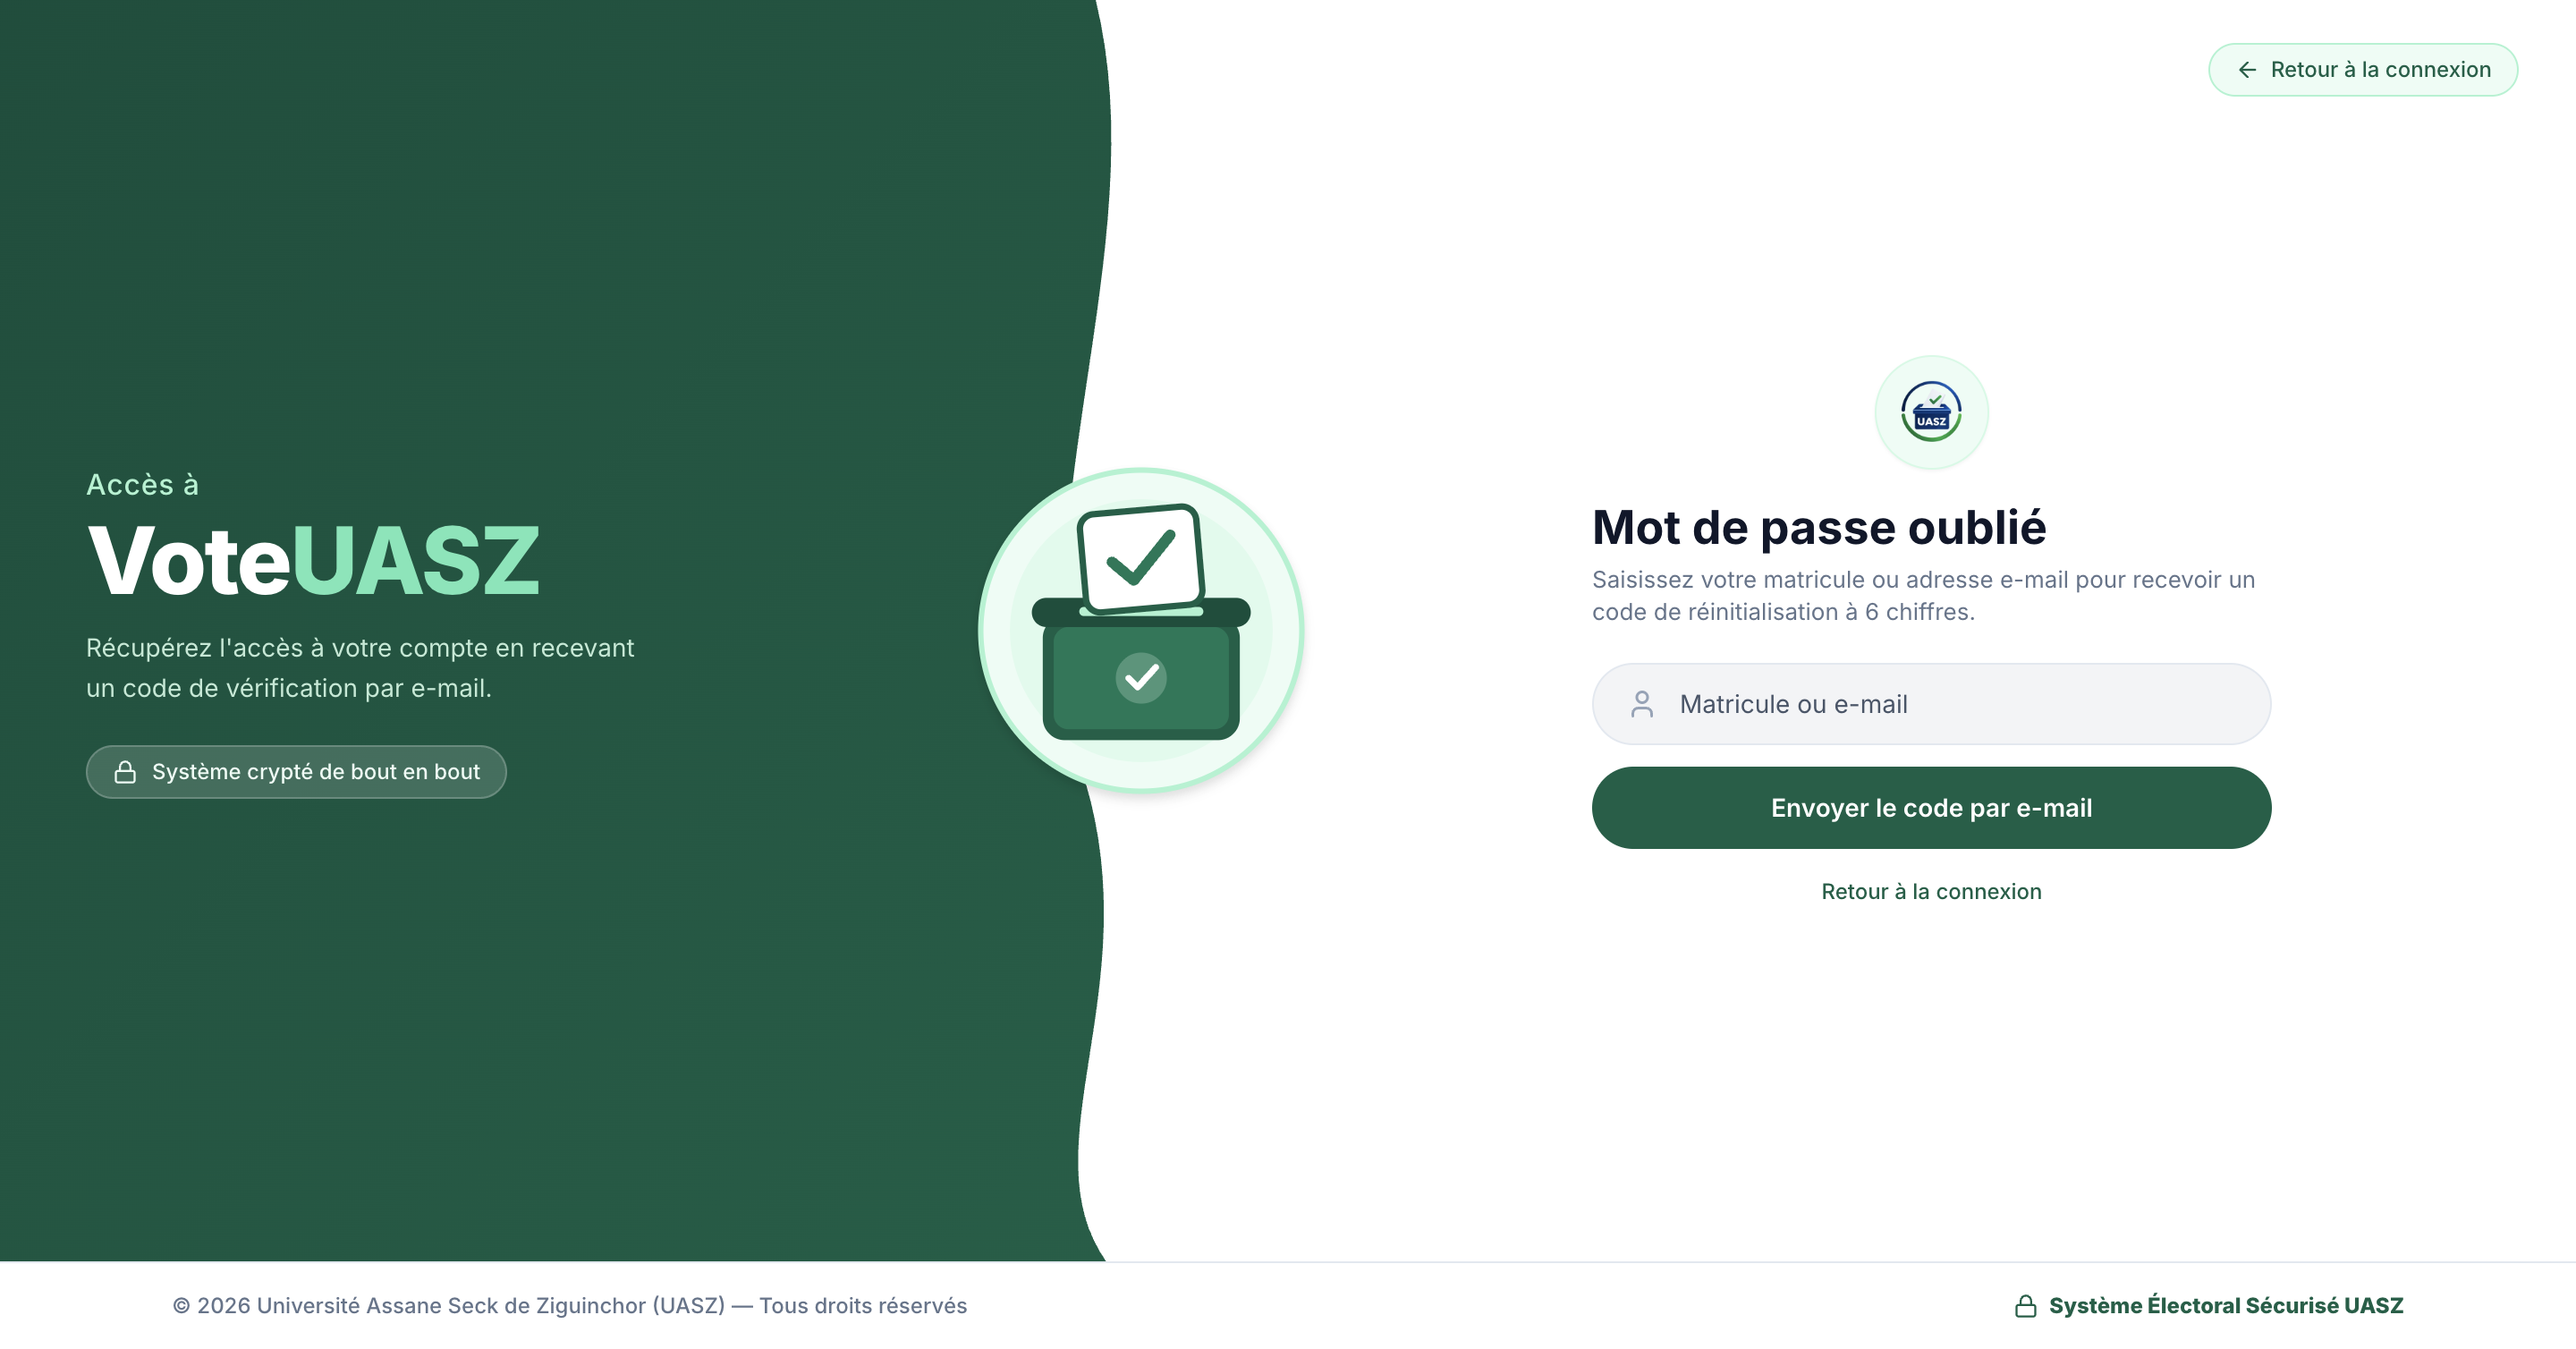
\includegraphics[width=\textwidth,height=0.42\textheight,keepaspectratio]{3-2-1-forgot-password.png}
        \caption{Demande de réinitialisation de mot de passe}
        \label{fig:forgot}
    \end{minipage}
\end{figure}

\begin{figure}[H]
    \centering
    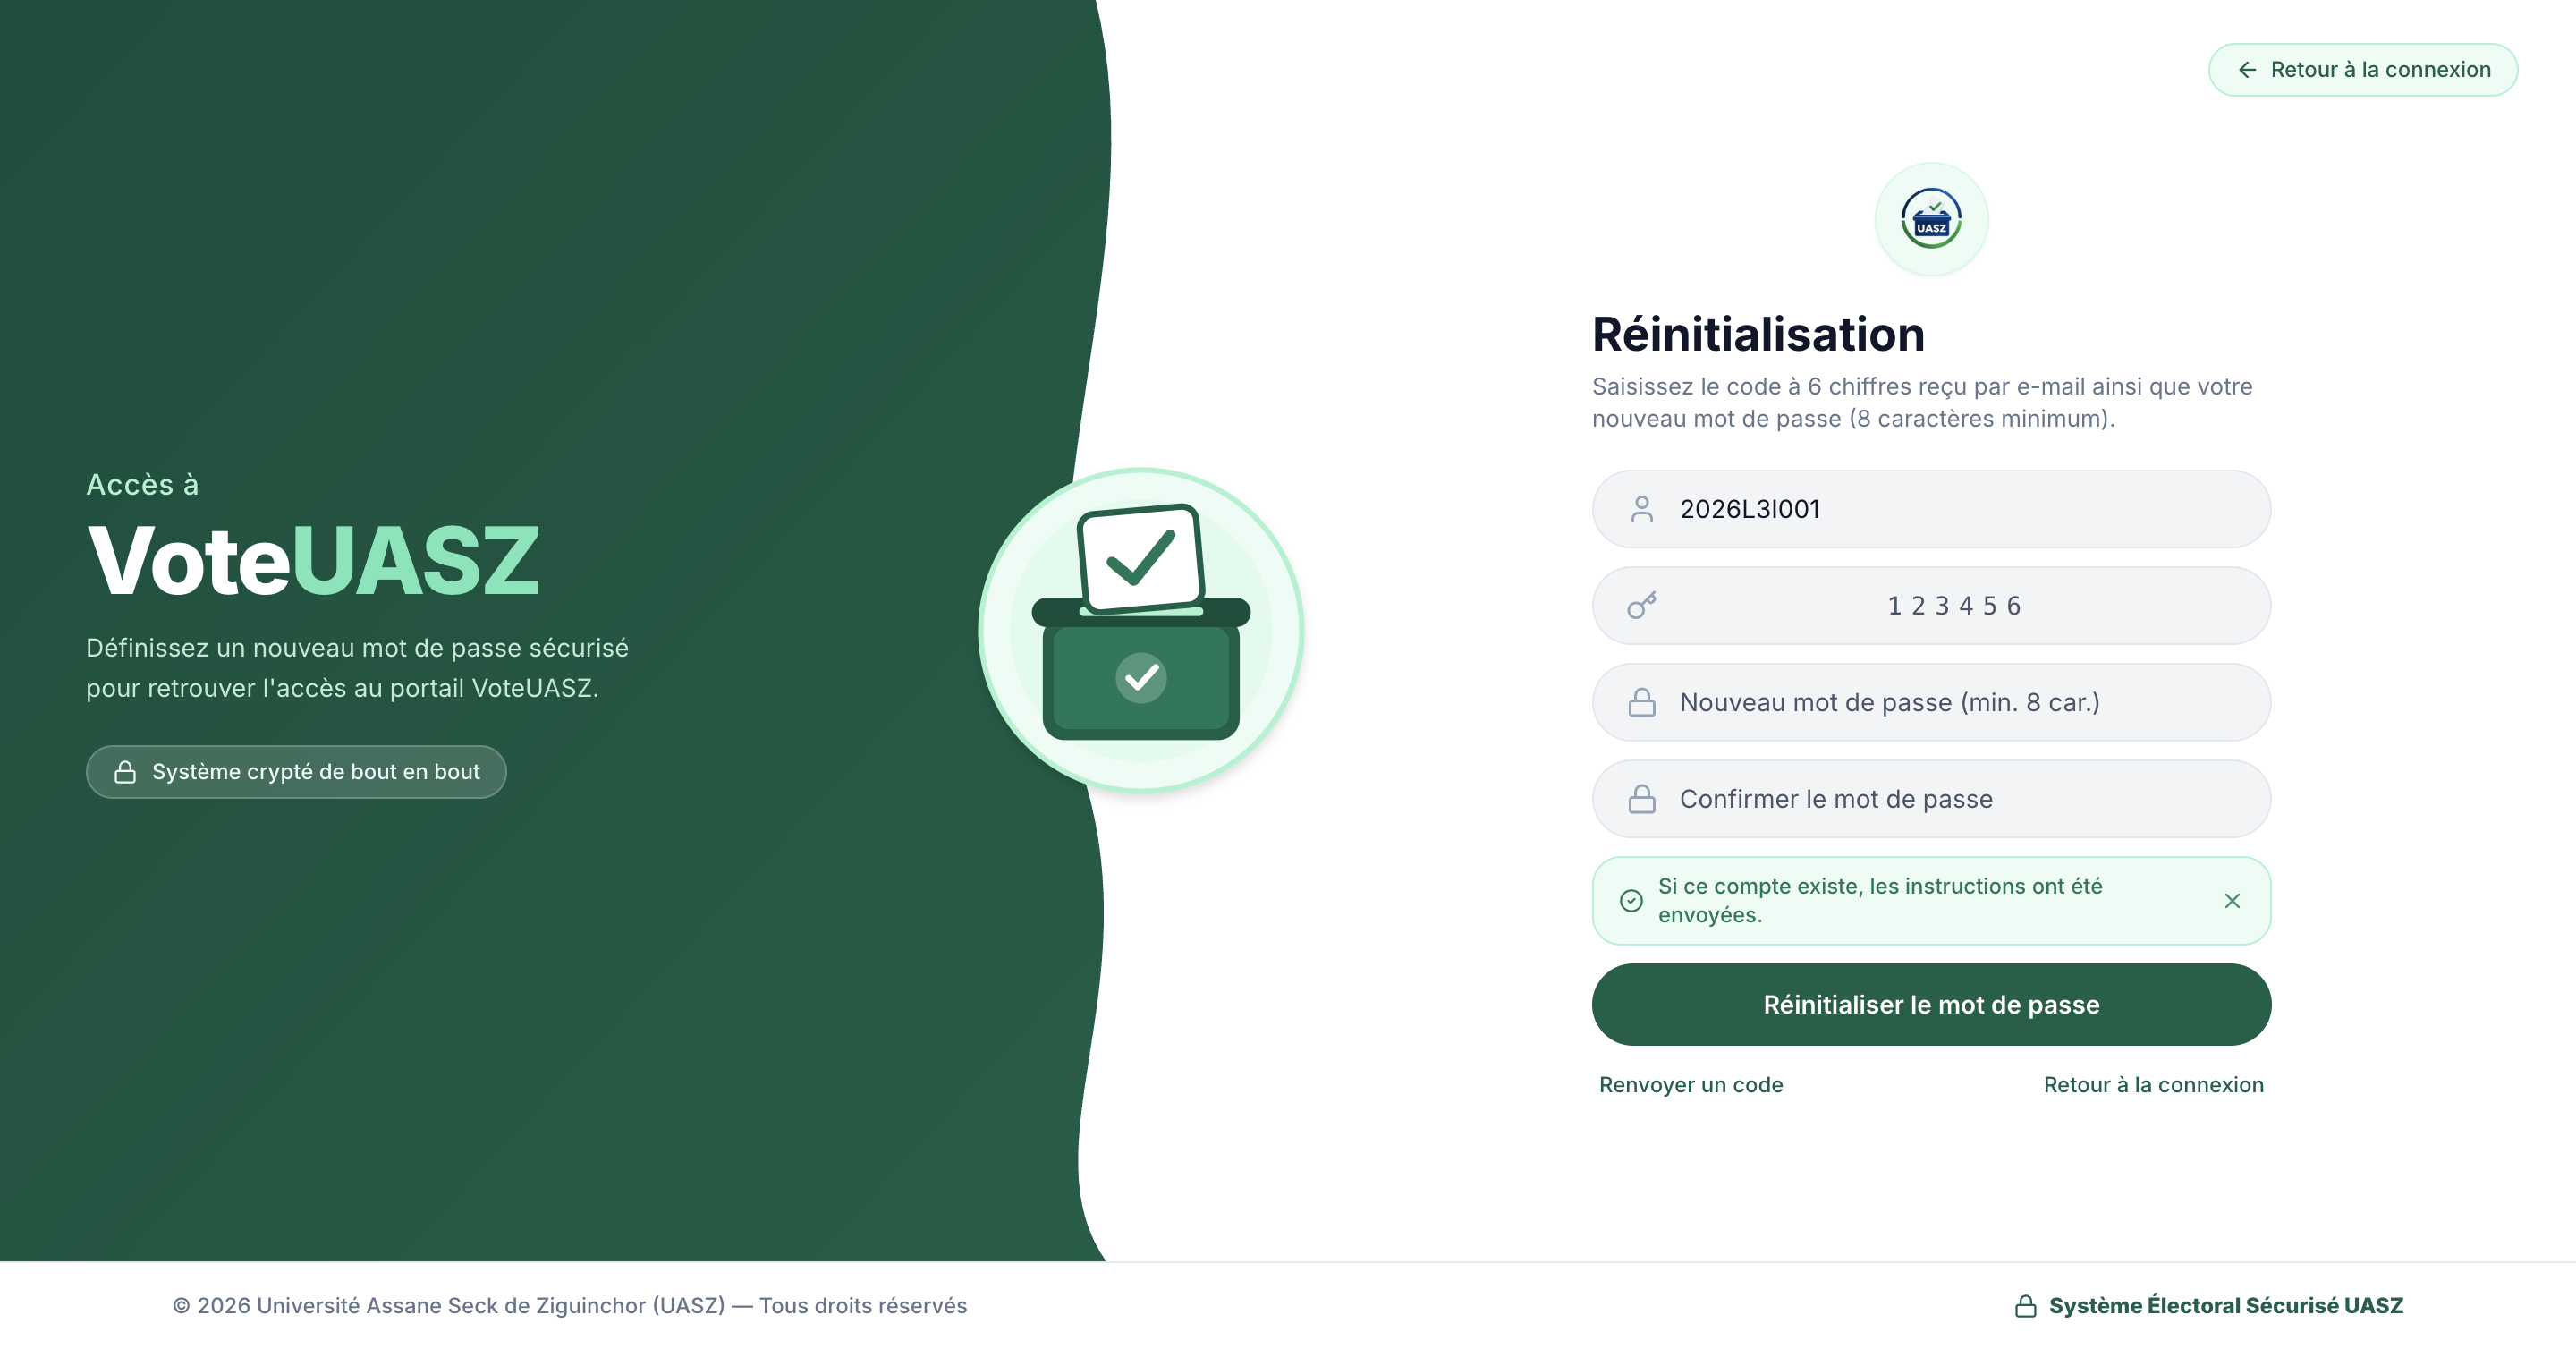
\includegraphics[width=0.85\textwidth,height=0.42\textheight,keepaspectratio]{3-2-1-reset-password.png}
    \caption{Saisie du code de réinitialisation et du nouveau mot de passe}
    \label{fig:reset}
\end{figure}

\subsection{Consultation des scrutins et vote sécurisé}
Les figures~\ref{fig:elec-tab}, \ref{fig:elec-cards} et~\ref{fig:elec-mob} présentent la liste des 5 scrutins (vues tableau, cartes et mobile). Les figures~\ref{fig:detail-stepper}, \ref{fig:detail-otp}, \ref{fig:mailhog-otp}, \ref{fig:detail-drawer}, \ref{fig:detail-results} et~\ref{fig:detail-mobile} montrent le stepper de vote en 3 étapes, l'e-mail OTP reçu dans MailHog, le drawer de campagne (photo, affiche, vidéo YouTube et texte long) et le graphique Chart.js des résultats en direct.

\begin{figure}[H]
    \centering
    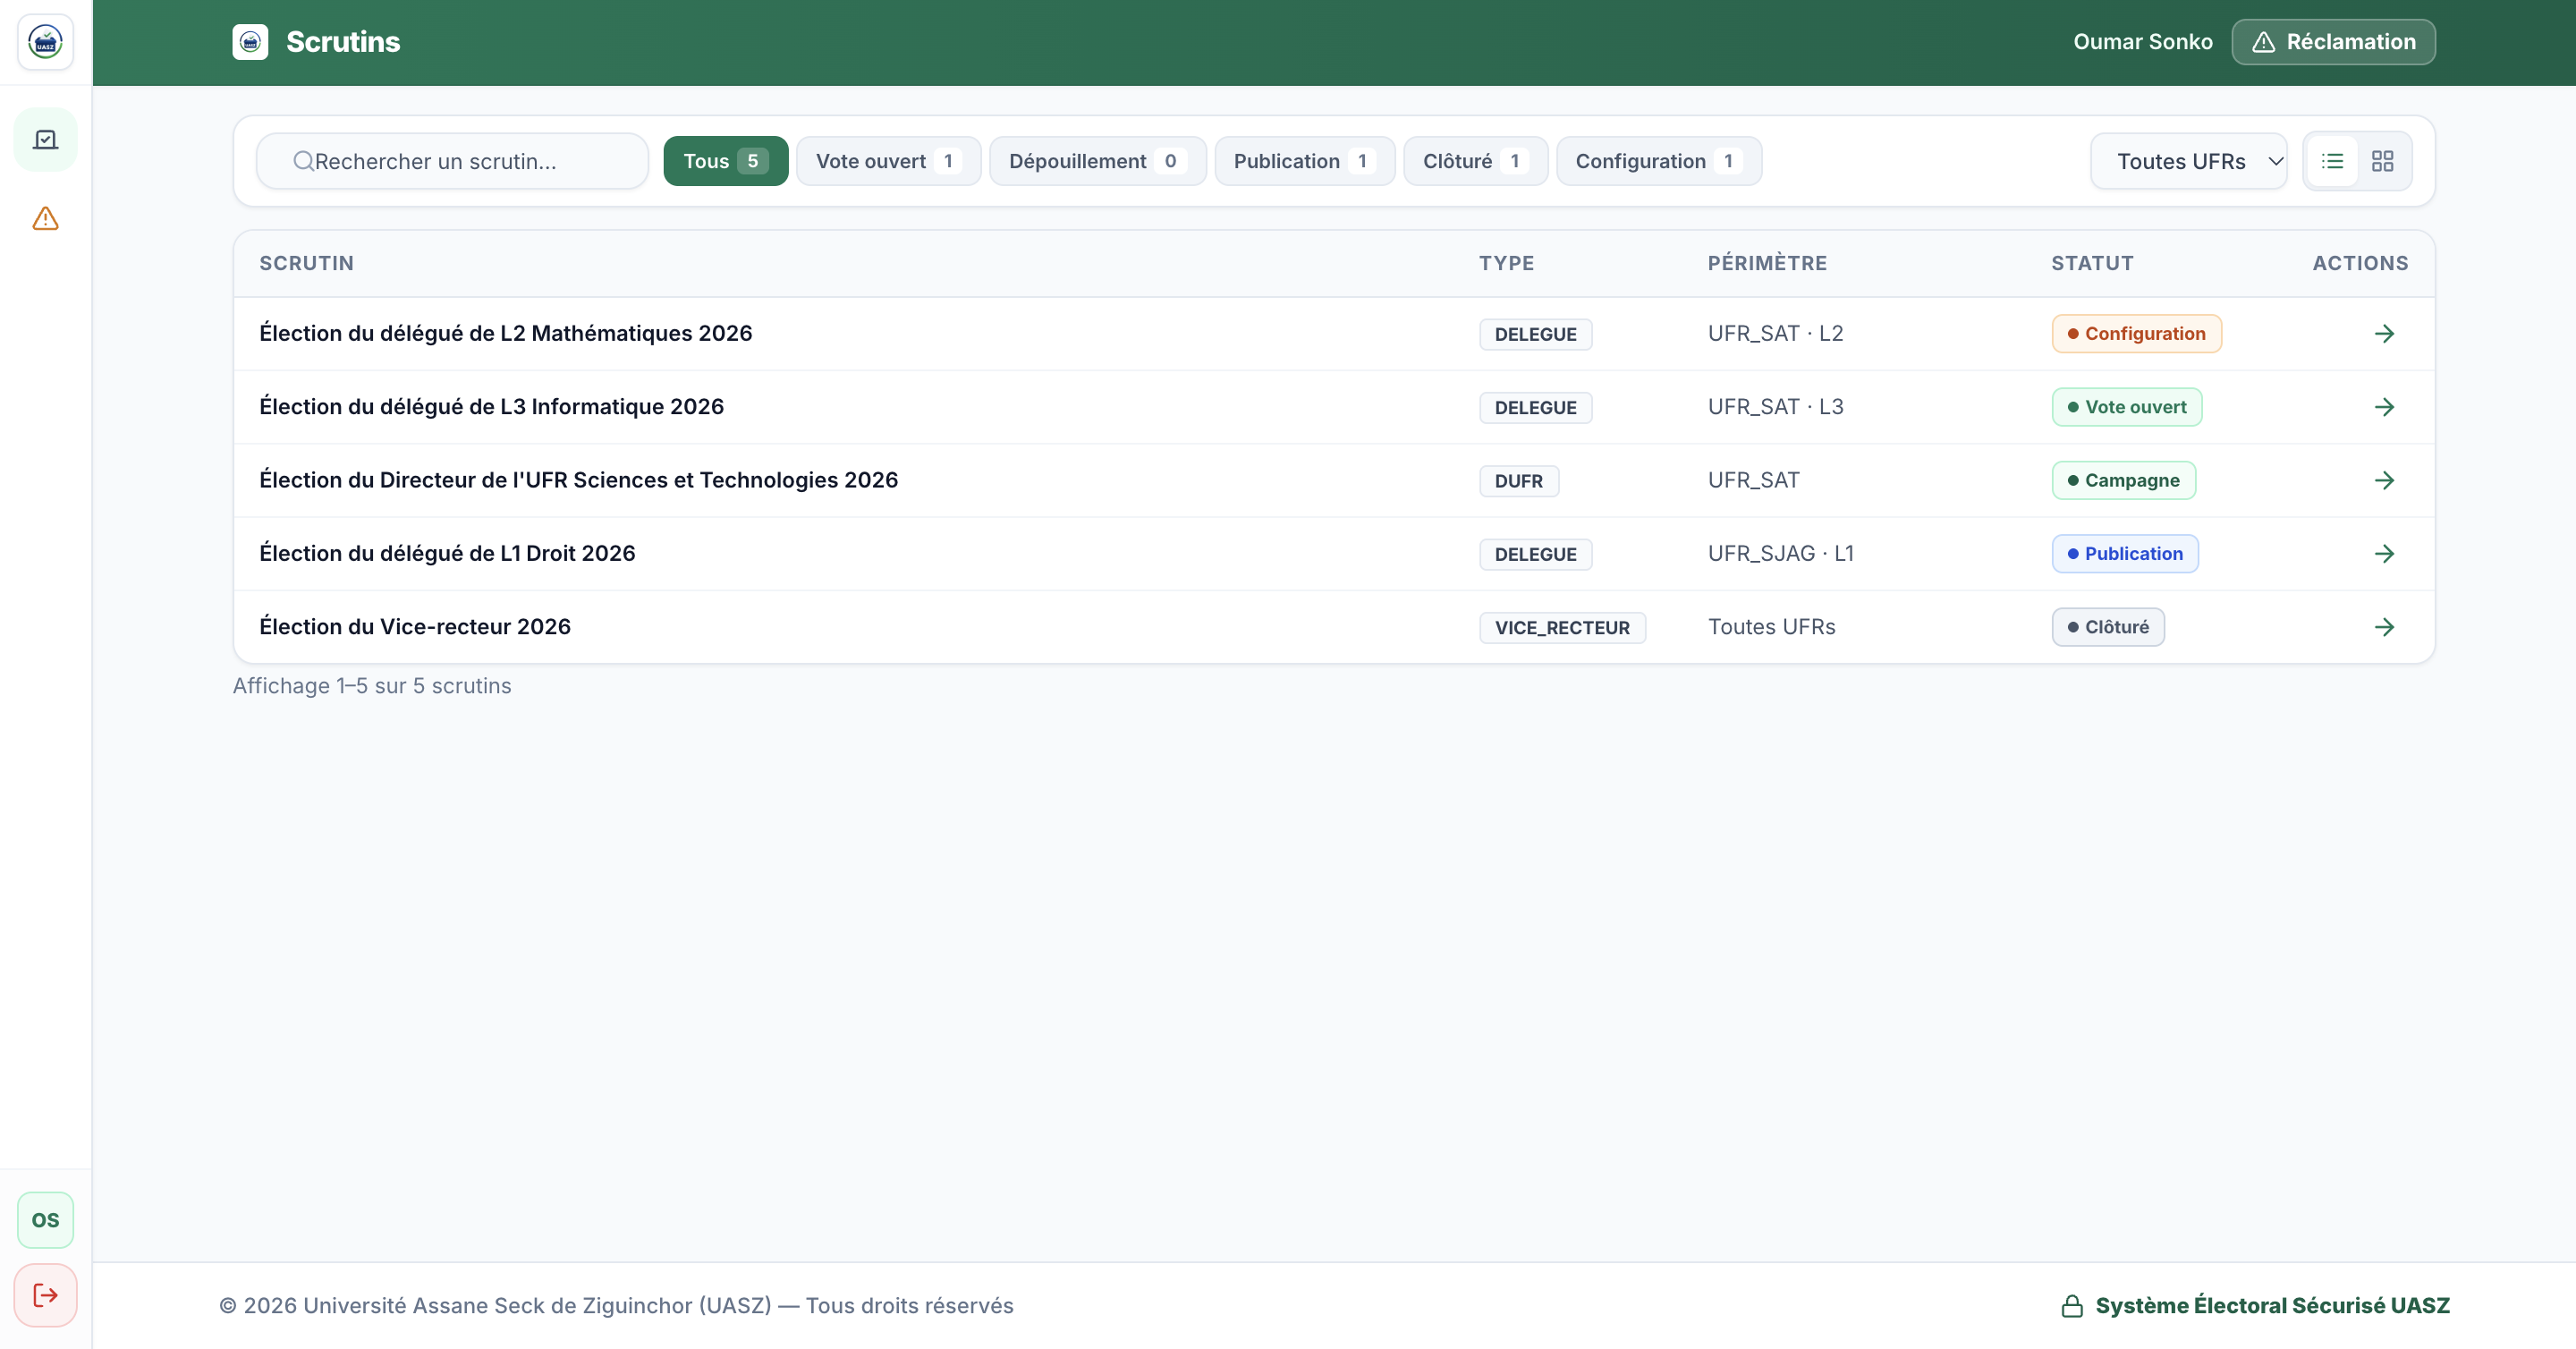
\includegraphics[width=0.92\textwidth,height=0.44\textheight,keepaspectratio]{3-2-2-elections-tableau.png}
    \caption{Liste des scrutins en vue tableau (\texttt{/elections})}
    \label{fig:elec-tab}
\end{figure}

\begin{figure}[H]
    \centering
    \begin{minipage}{0.62\textwidth}
        \centering
        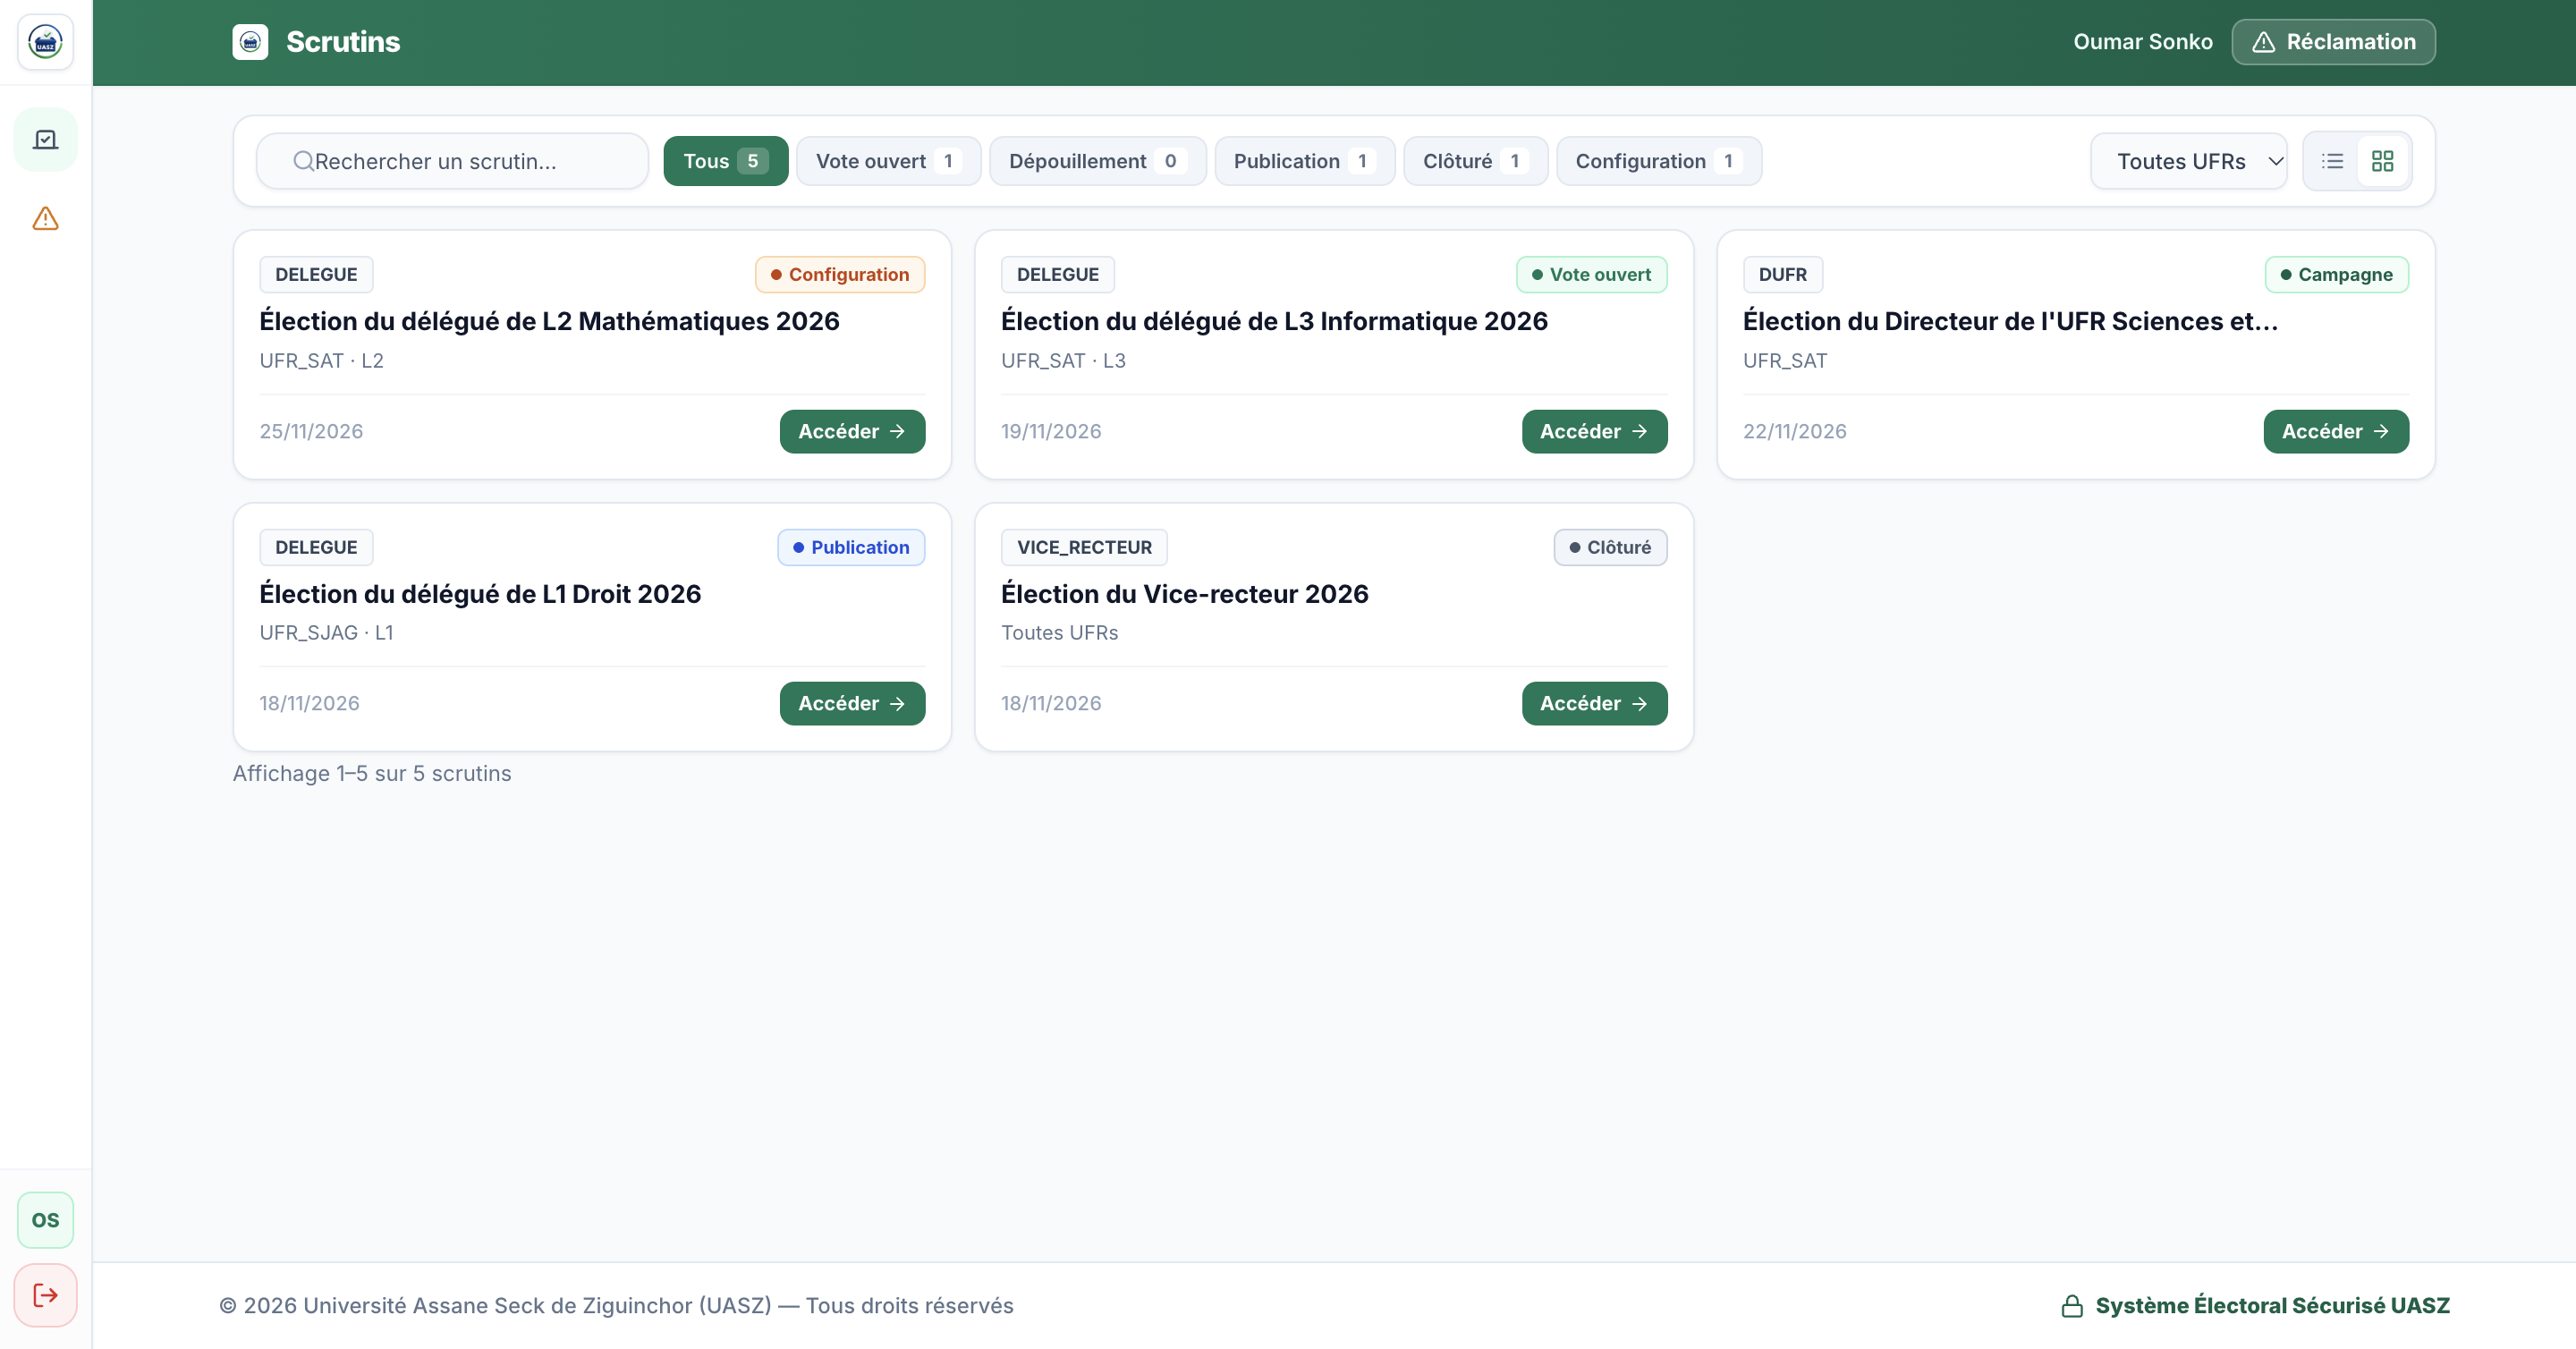
\includegraphics[width=\textwidth,height=0.42\textheight,keepaspectratio]{3-2-2-elections-cartes.png}
        \caption{Liste des scrutins en vue cartes}
        \label{fig:elec-cards}
    \end{minipage}
    \hfill
    \begin{minipage}{0.34\textwidth}
        \centering
        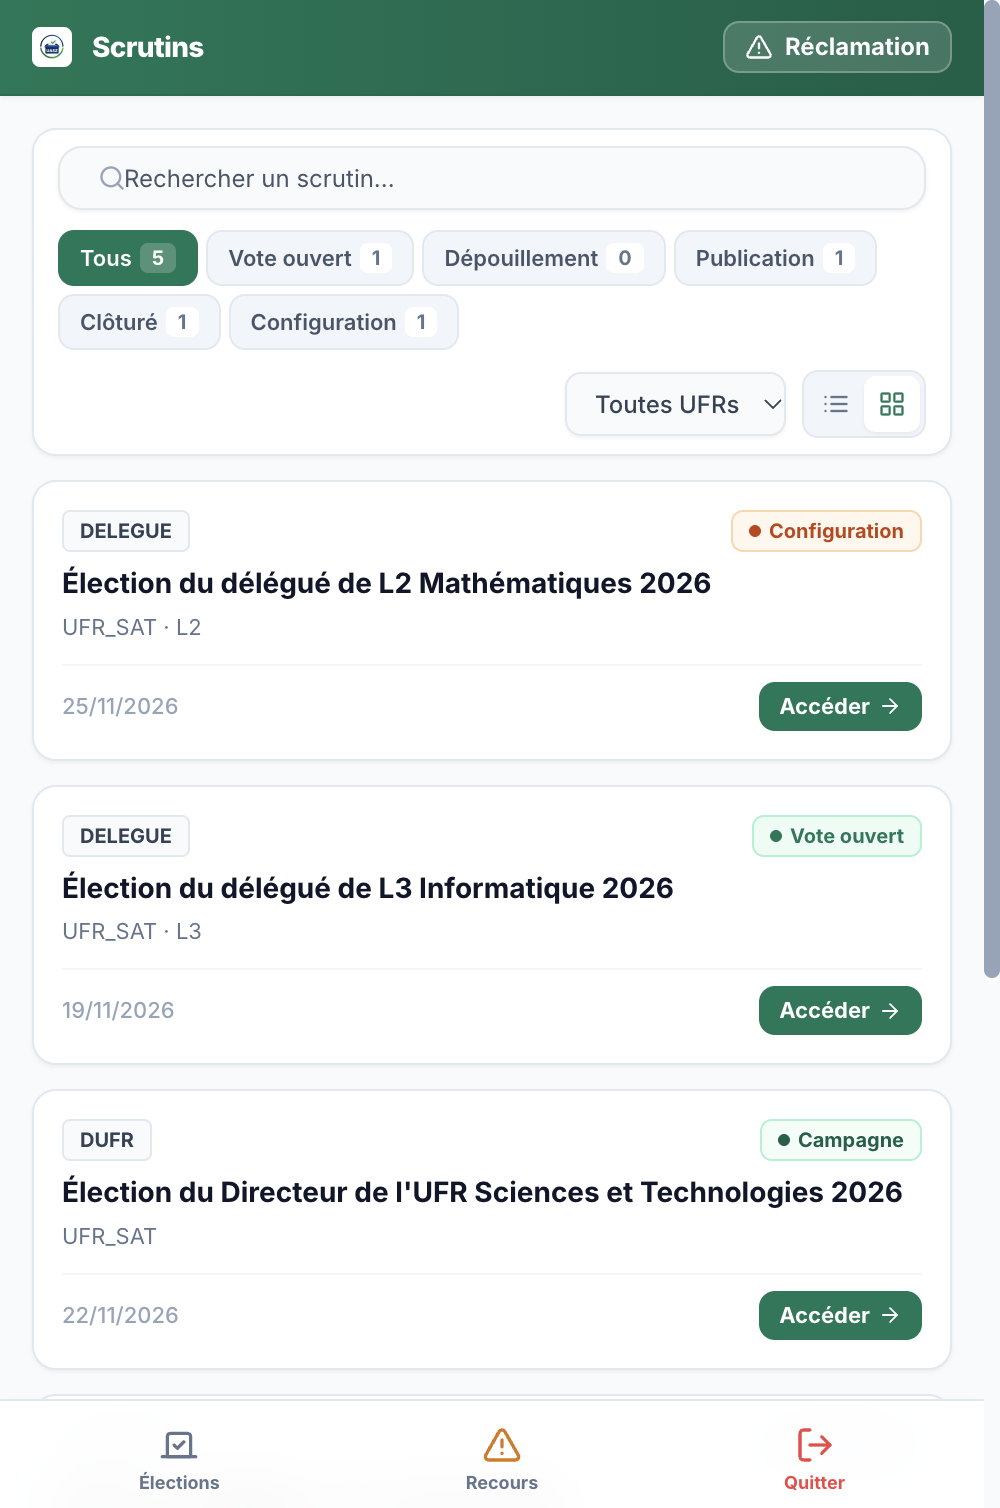
\includegraphics[width=\textwidth,height=0.42\textheight,keepaspectratio]{3-2-2-elections-mobile.png}
        \caption{Vue mobile (\texttt{390x844})}
        \label{fig:elec-mob}
    \end{minipage}
\end{figure}

\begin{figure}[H]
    \centering
    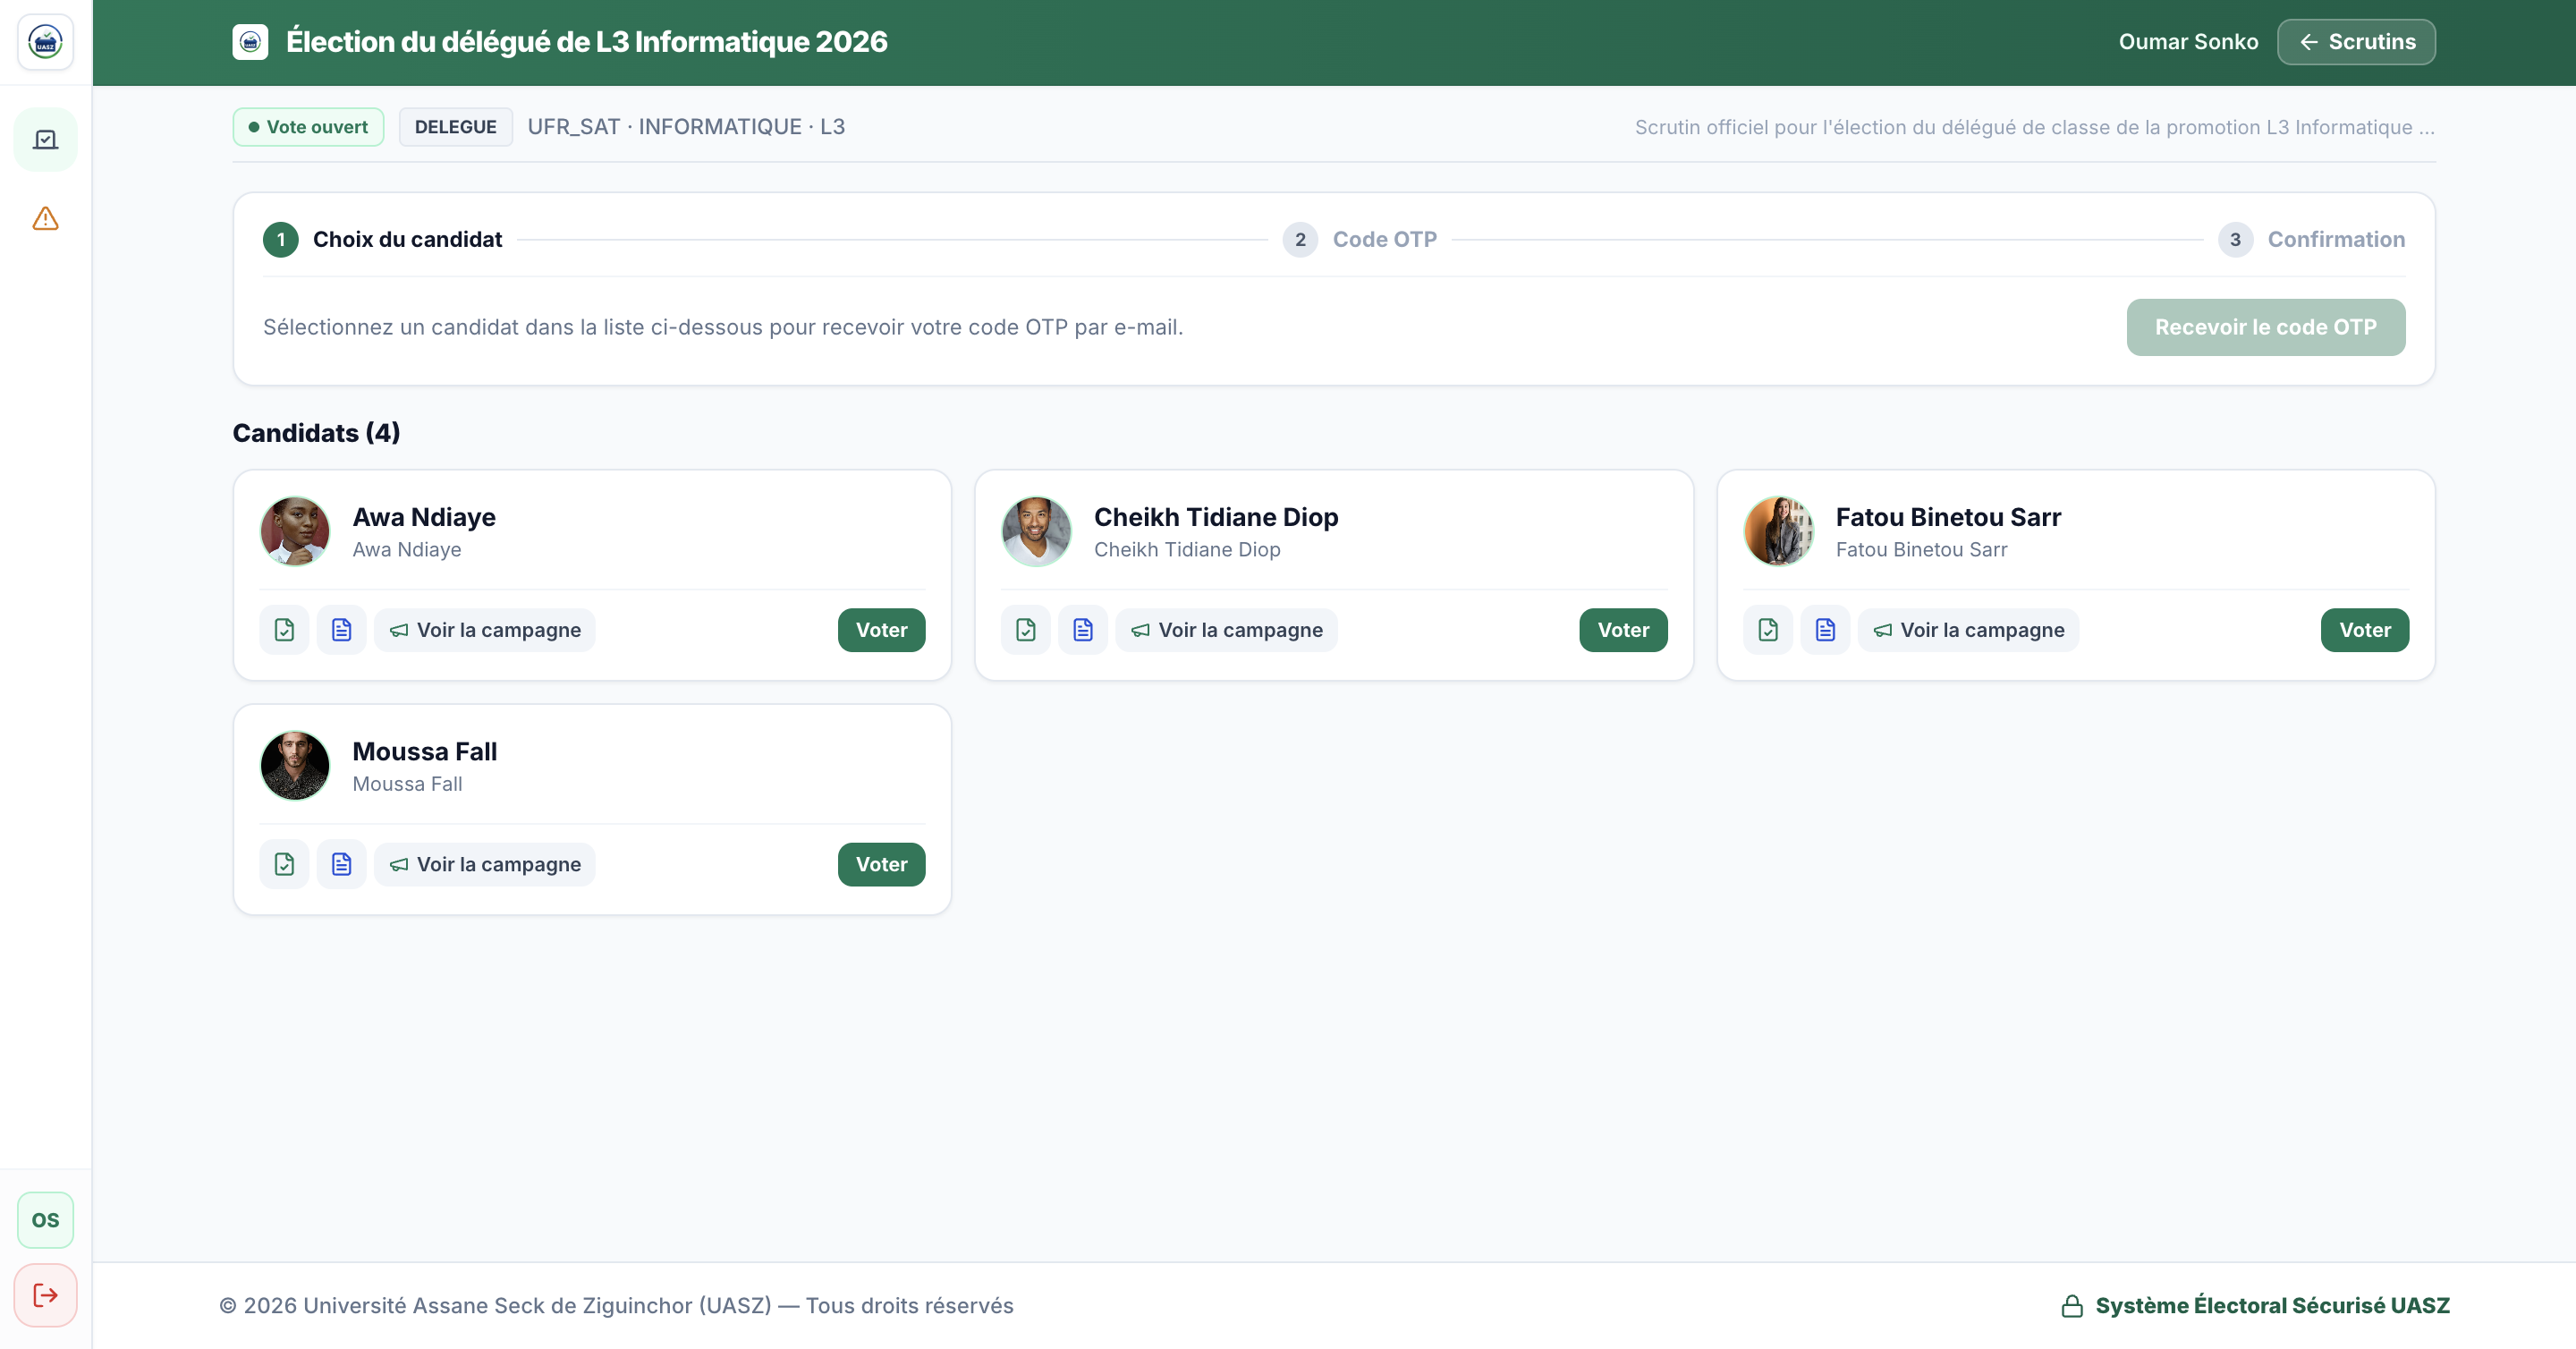
\includegraphics[width=0.92\textwidth,height=0.44\textheight,keepaspectratio]{3-2-3-election-detail-stepper.png}
    \caption{Détail d'élection ouverte : stepper de vote en 3 étapes (\texttt{L3 Informatique 2026})}
    \label{fig:detail-stepper}
\end{figure}

\begin{figure}[H]
    \centering
    \begin{minipage}{0.48\textwidth}
        \centering
        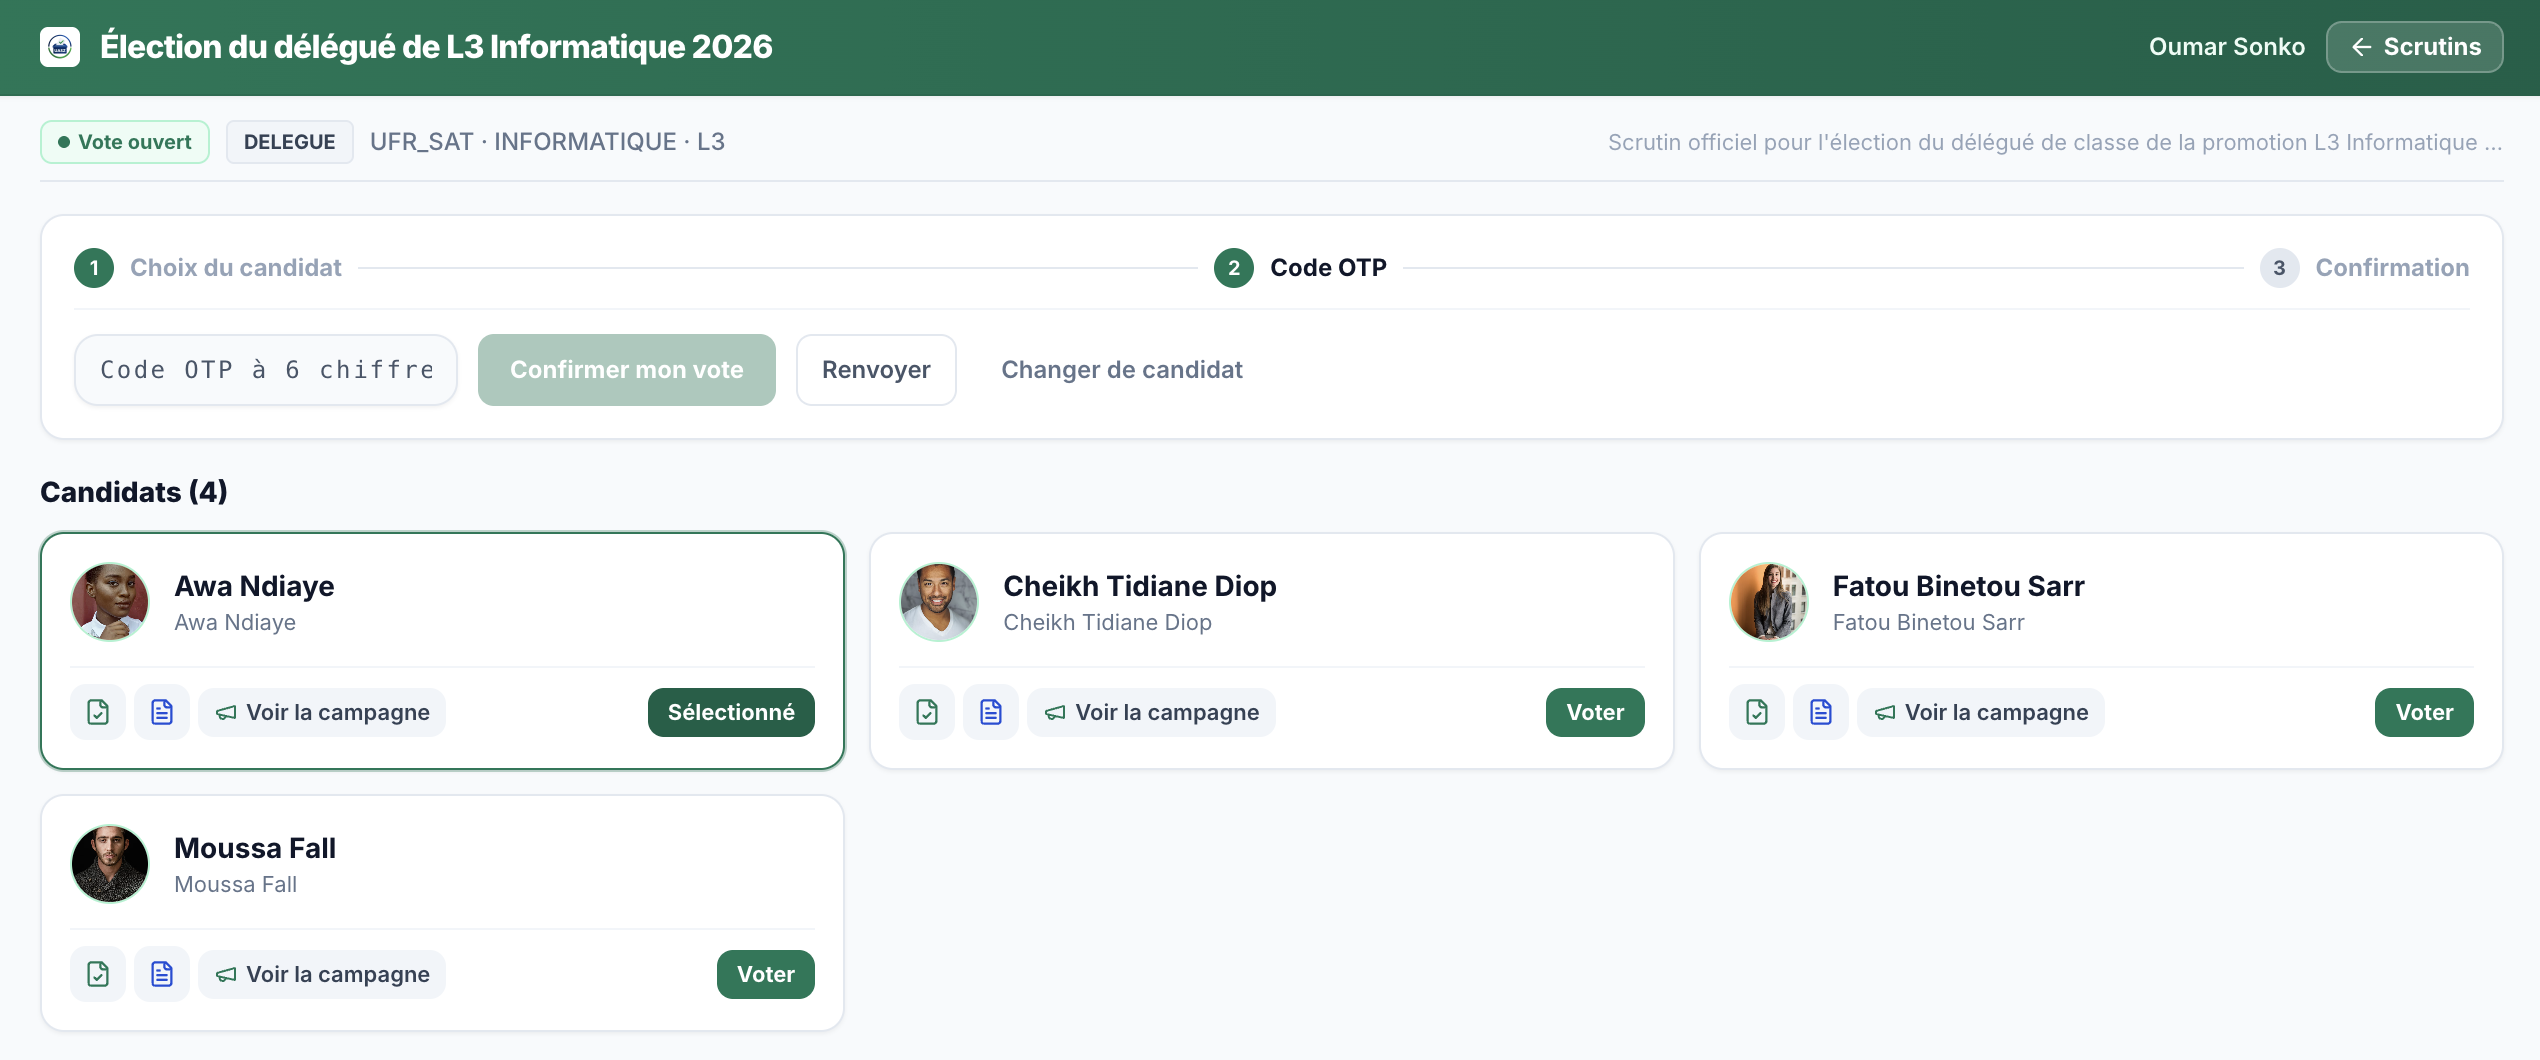
\includegraphics[width=\textwidth,height=0.38\textheight,keepaspectratio]{3-2-3-election-detail-otp.png}
        \caption{Étape de saisie du code OTP}
        \label{fig:detail-otp}
    \end{minipage}
    \hfill
    \begin{minipage}{0.48\textwidth}
        \centering
        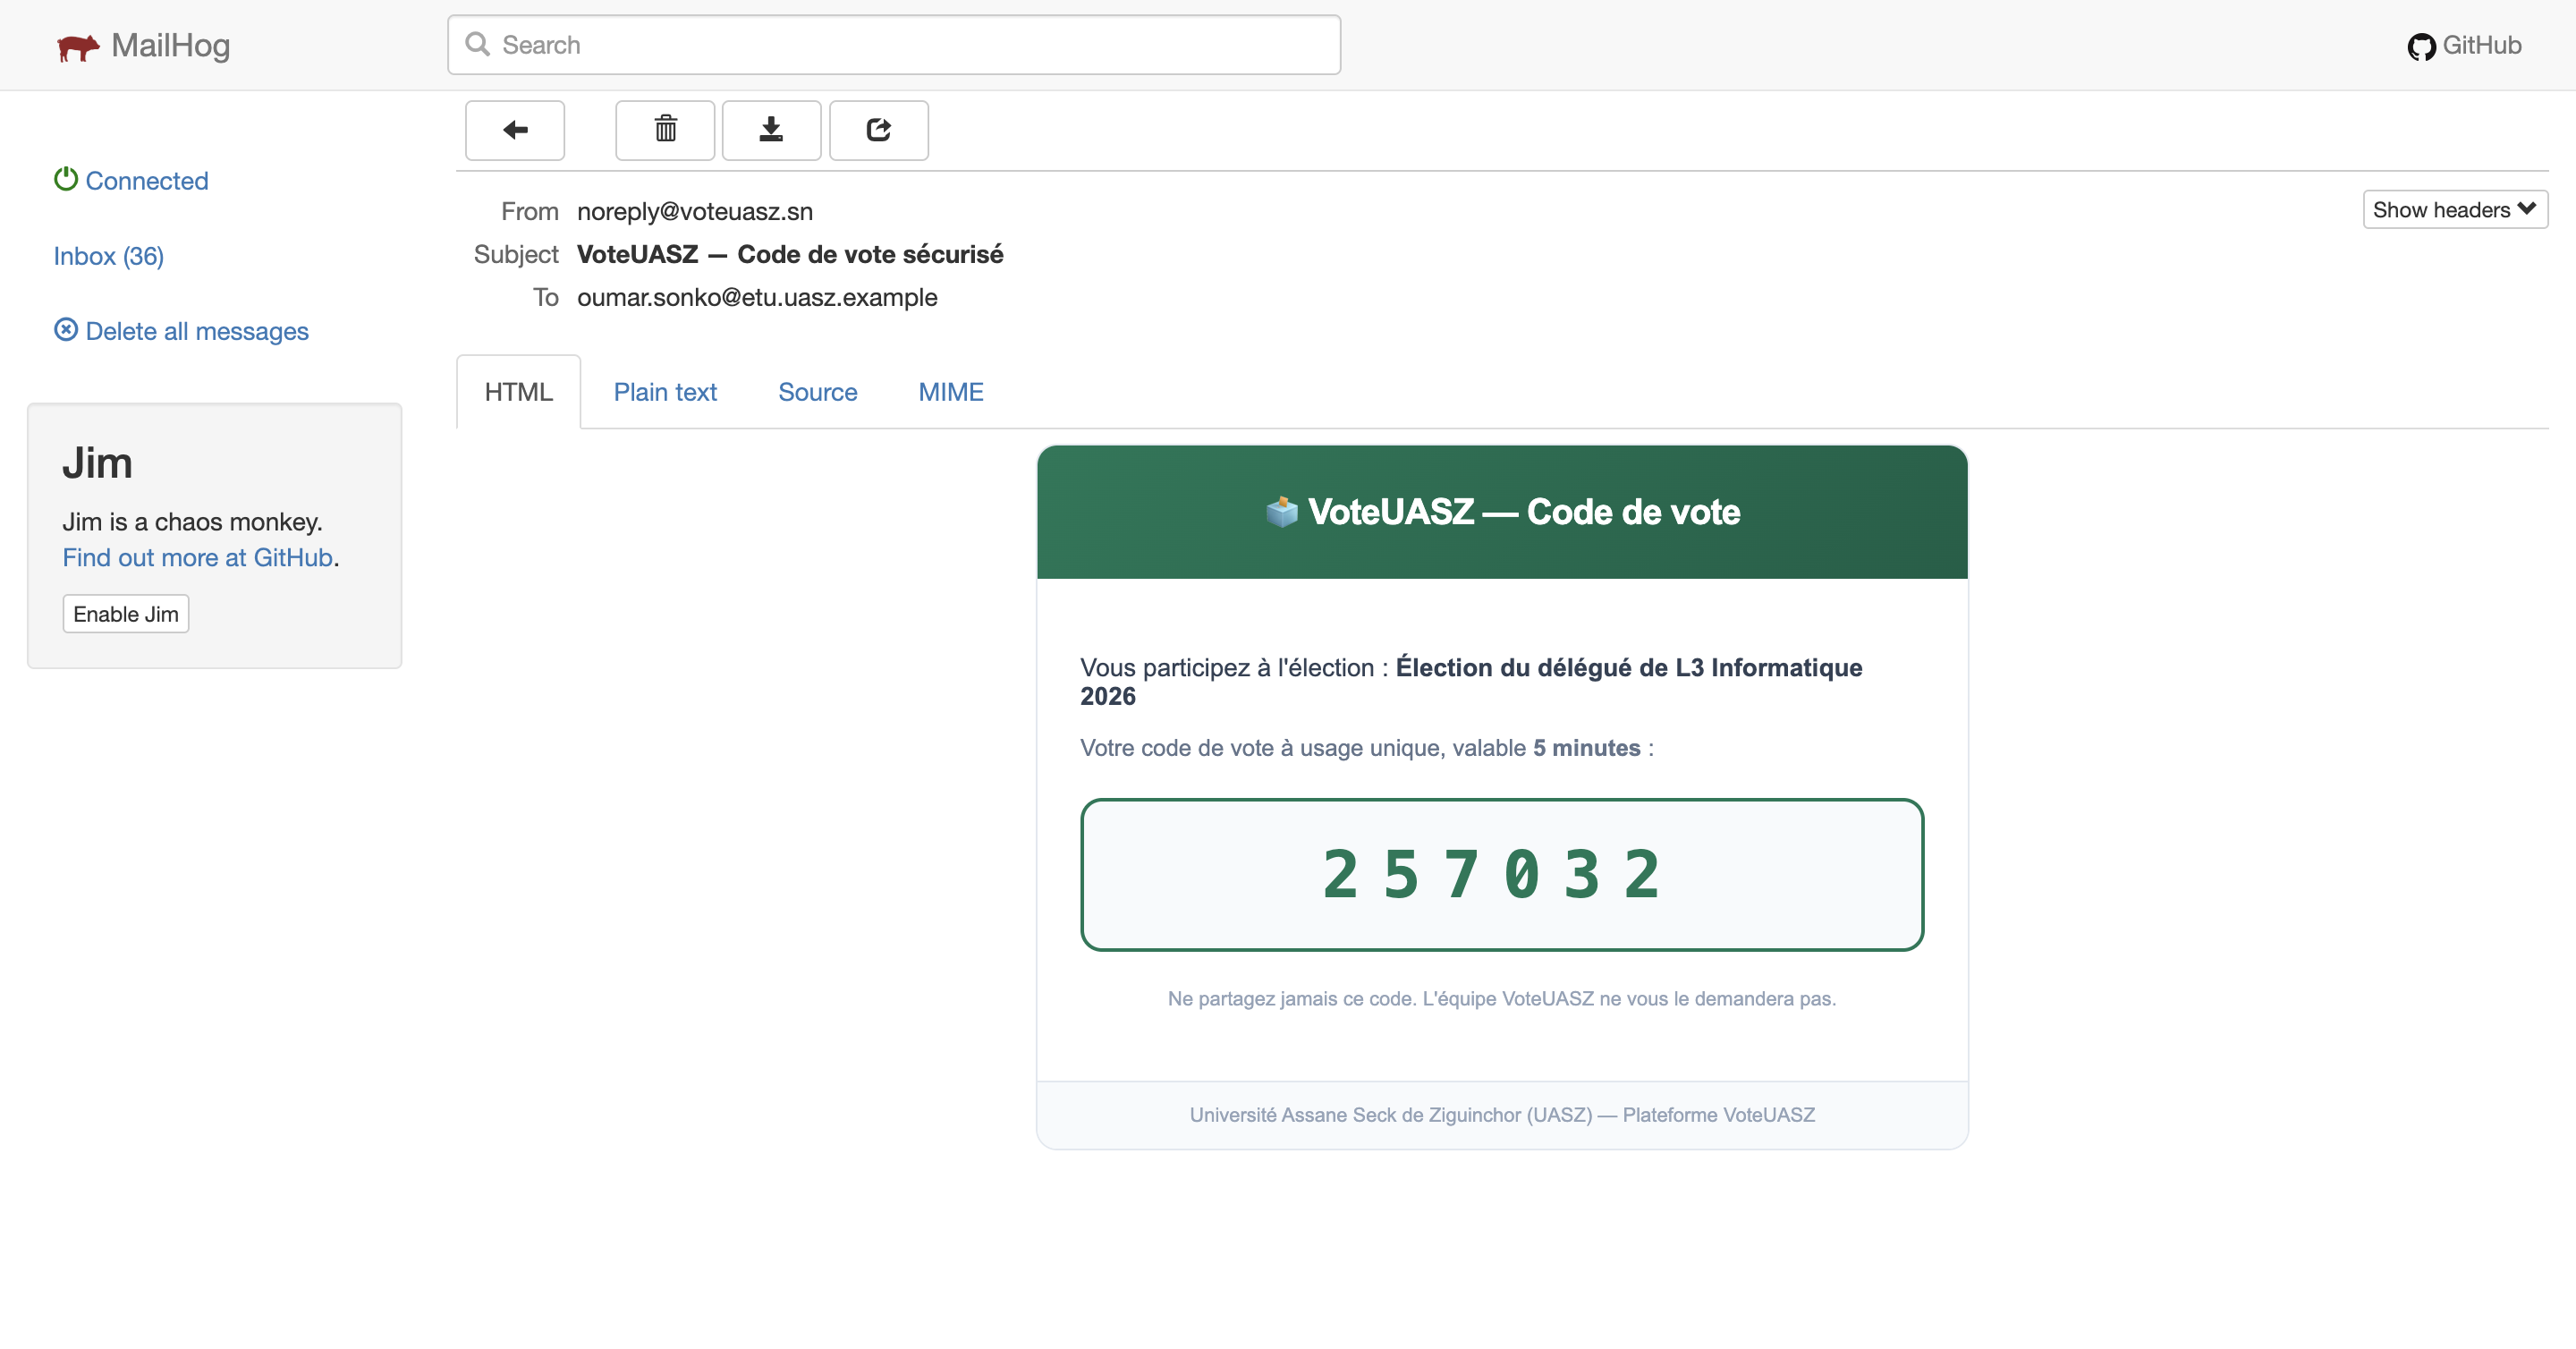
\includegraphics[width=\textwidth,height=0.38\textheight,keepaspectratio]{3-2-4-mailhog-otp.png}
        \caption{E-mail OTP reçu dans MailHog}
        \label{fig:mailhog-otp}
    \end{minipage}
\end{figure}

\begin{figure}[H]
    \centering
    \begin{minipage}{0.62\textwidth}
        \centering
        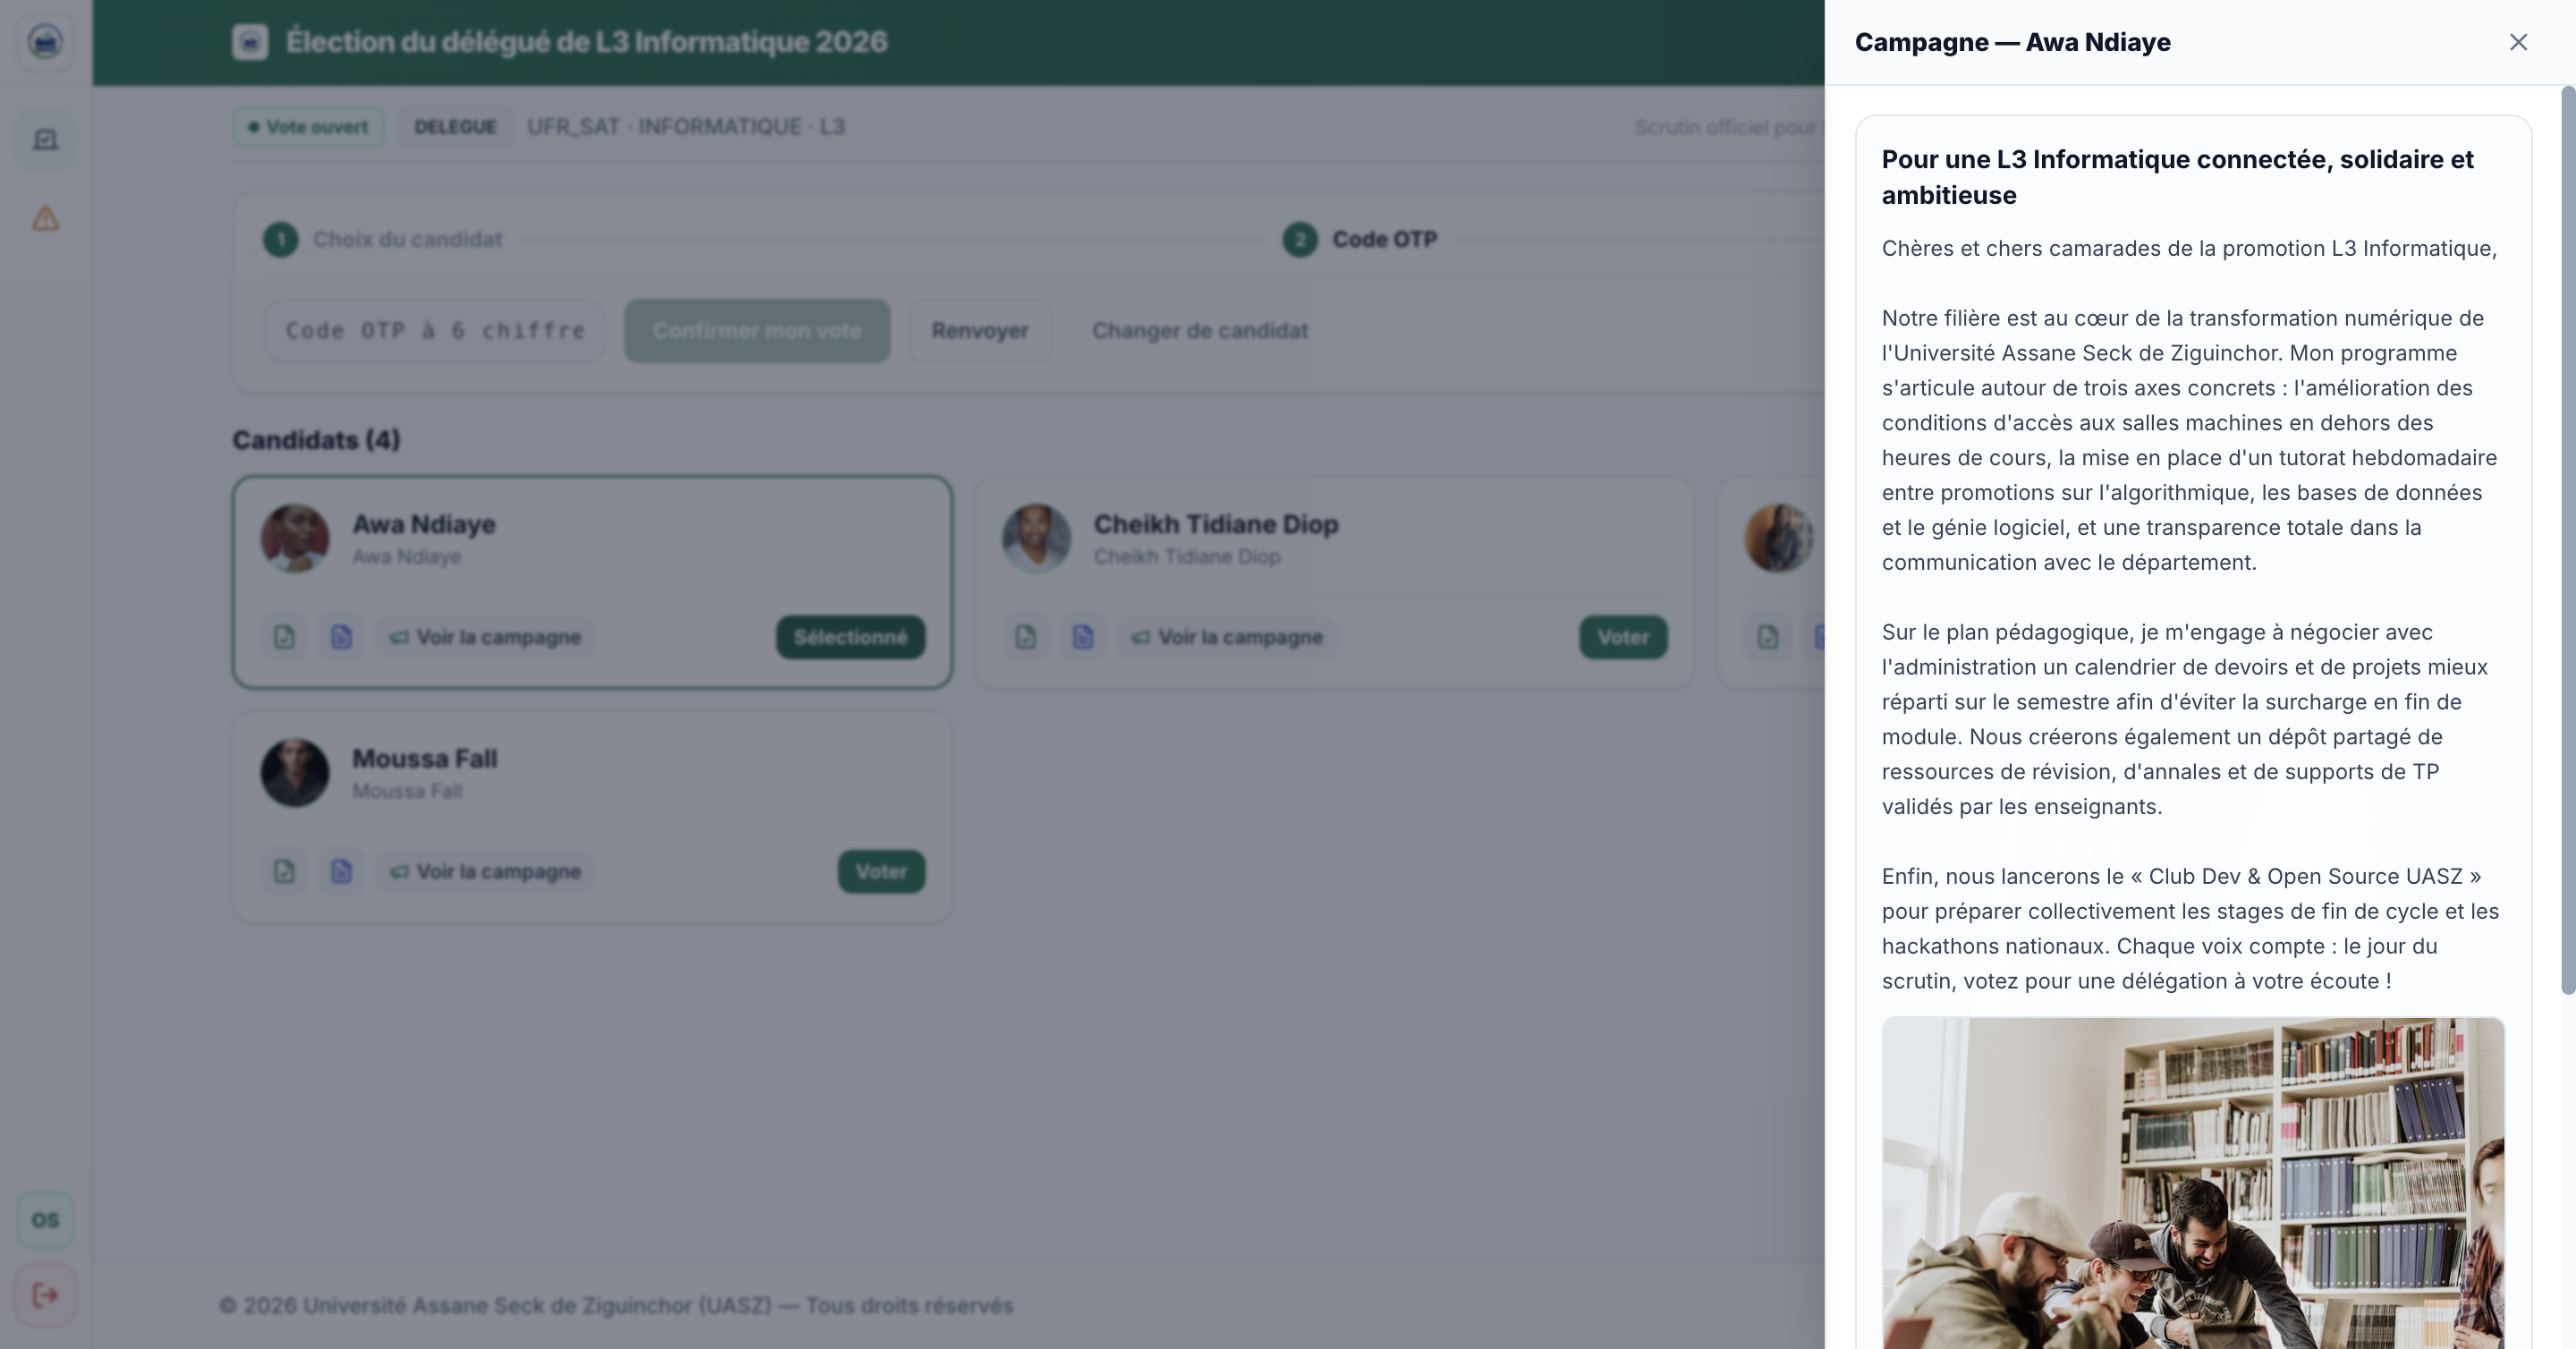
\includegraphics[width=\textwidth,height=0.42\textheight,keepaspectratio]{3-2-3-election-detail-drawer.png}
        \caption{Drawer de campagne (photo, affiche, vidéo YouTube et programme)}
        \label{fig:detail-drawer}
    \end{minipage}
    \hfill
    \begin{minipage}{0.34\textwidth}
        \centering
        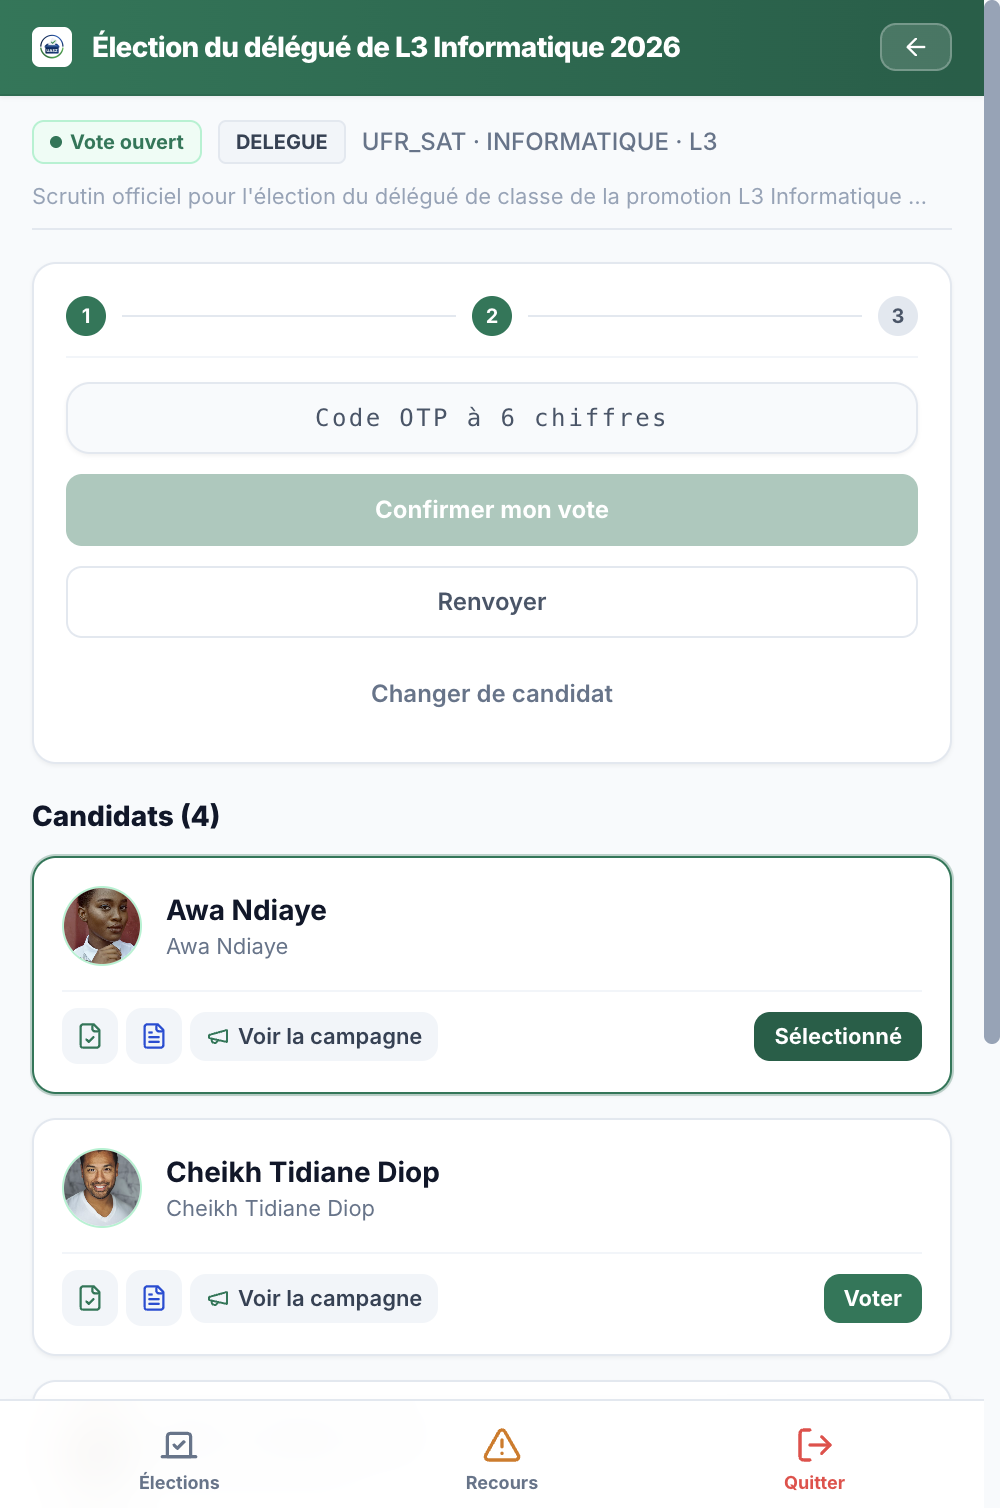
\includegraphics[width=\textwidth,height=0.42\textheight,keepaspectratio]{3-2-3-election-detail-mobile.png}
        \caption{Détail mobile (\texttt{390x844})}
        \label{fig:detail-mobile}
    \end{minipage}
\end{figure}

\begin{figure}[H]
    \centering
    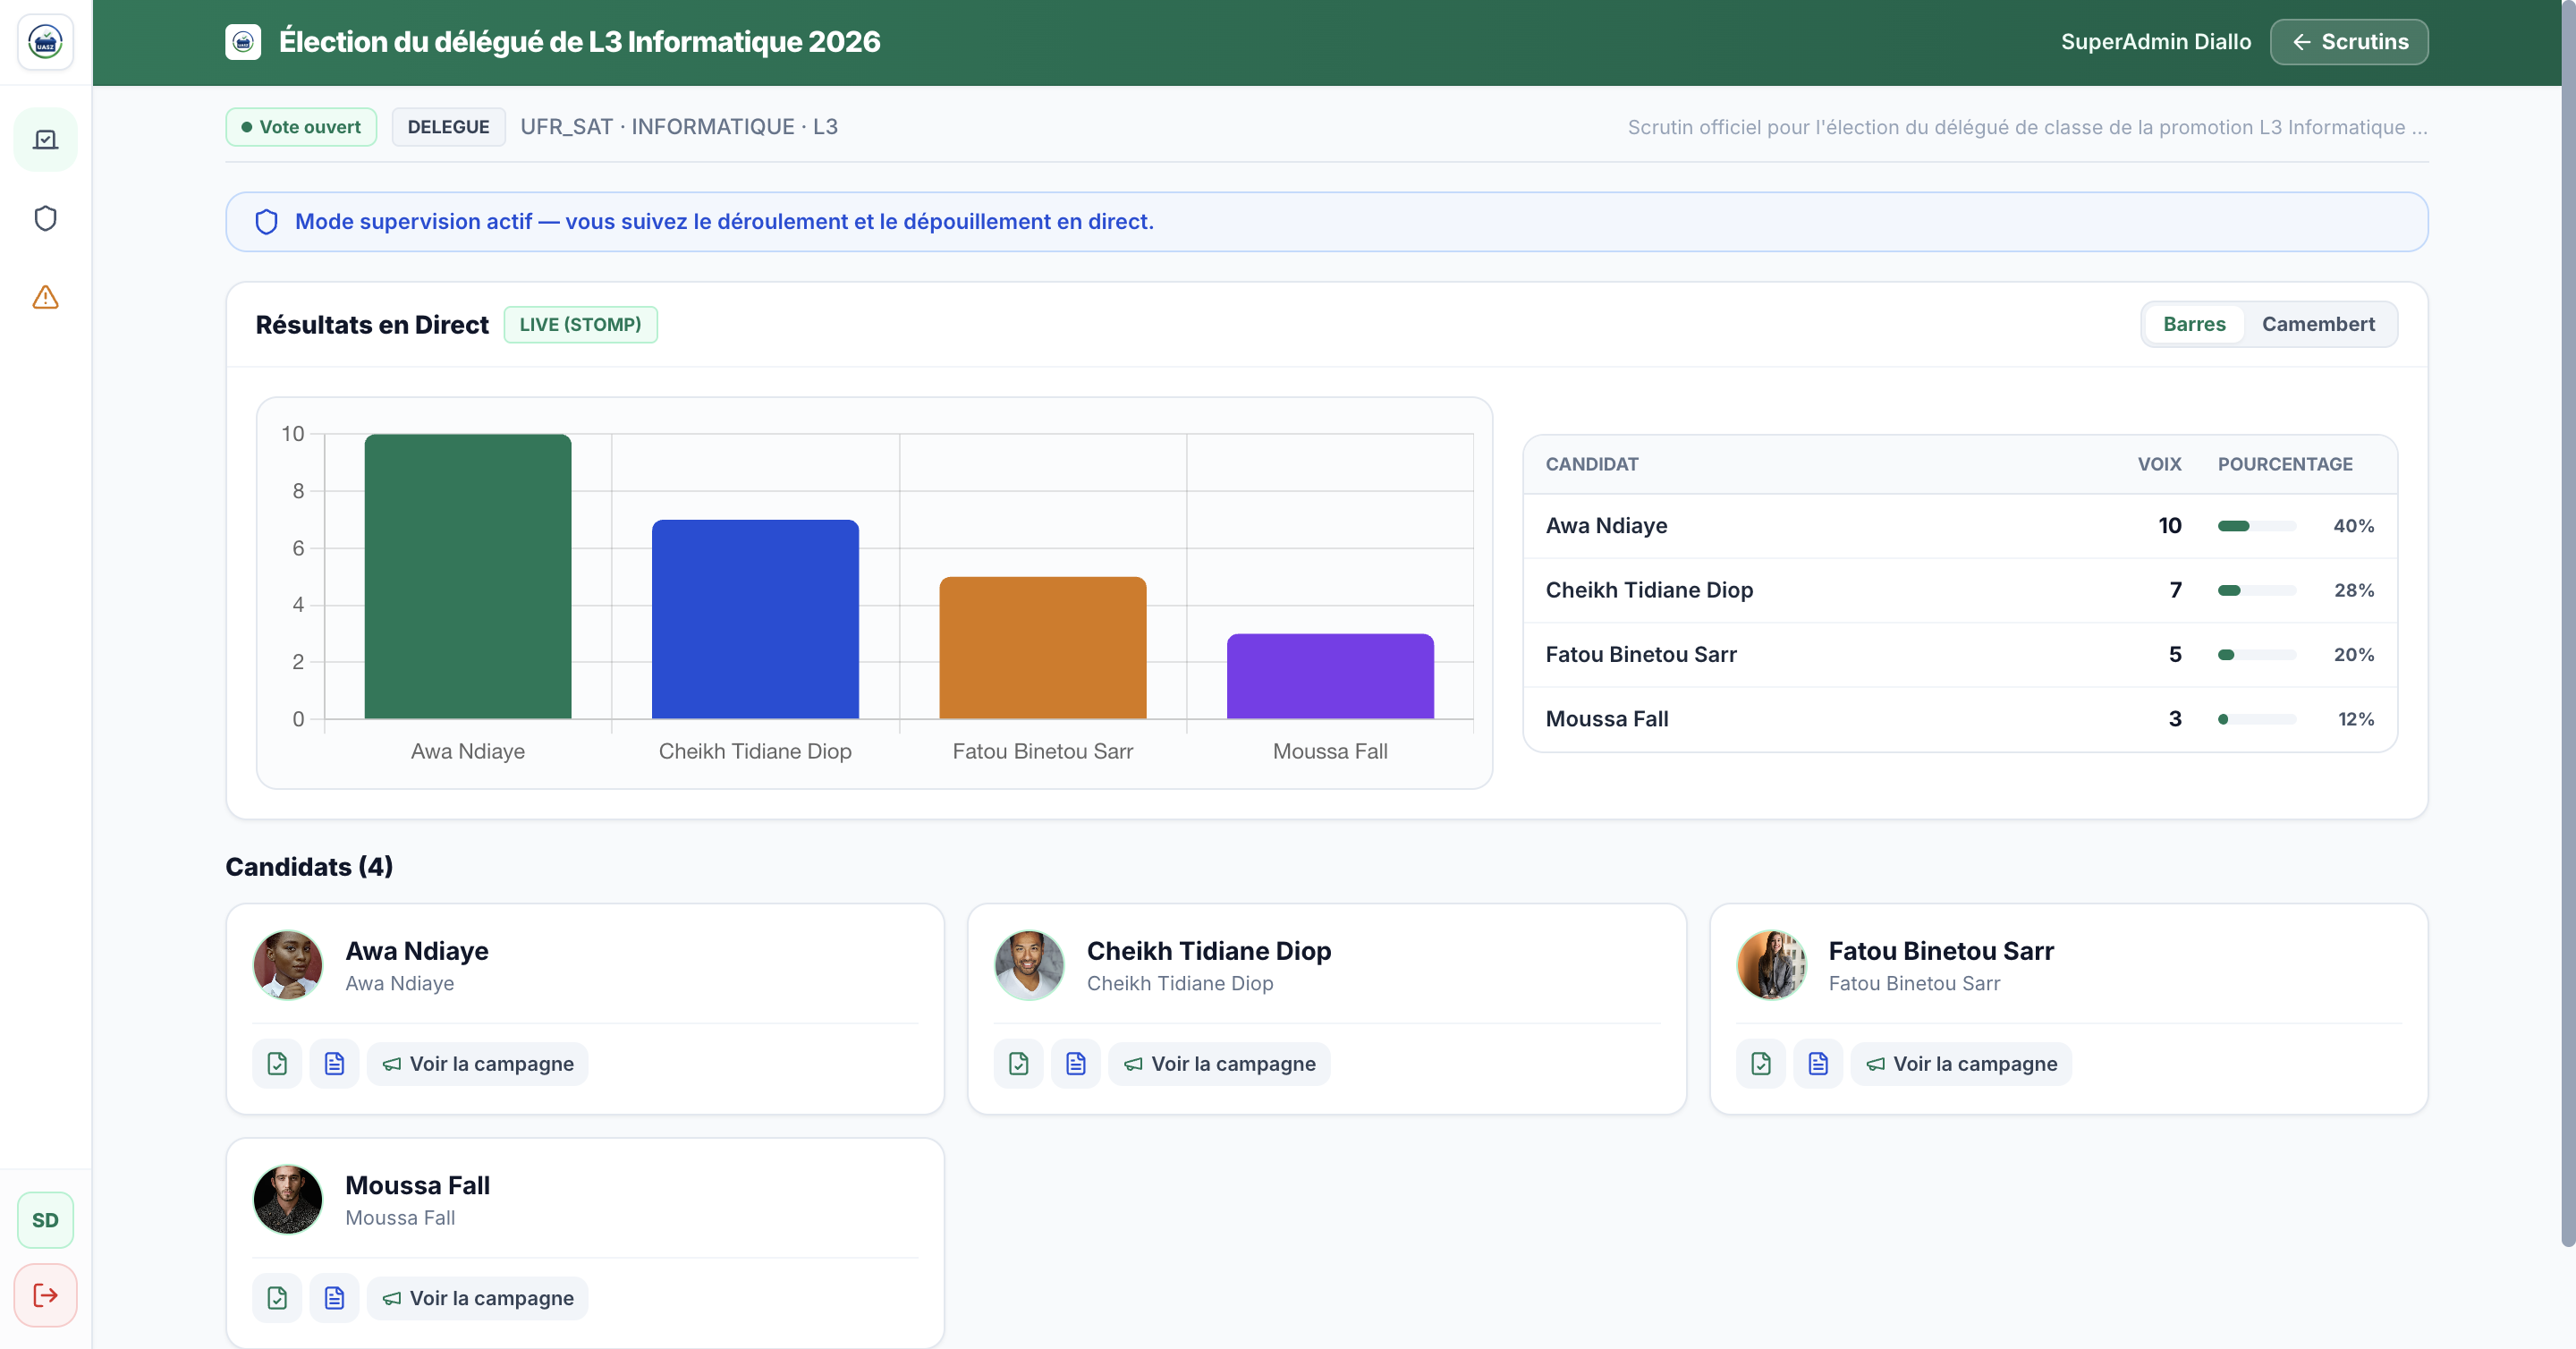
\includegraphics[width=0.92\textwidth,height=0.44\textheight,keepaspectratio]{3-2-3-election-detail-results-live.png}
    \caption{Résultats en direct à 4 candidats avec graphique Chart.js affiché automatiquement}
    \label{fig:detail-results}
\end{figure}

\subsection{Administration, Commission, Candidat, Réclamations et PV PDF}
Les figures~\ref{fig:admin-scrutins} à~\ref{fig:swagger} présentent l'espace Super-Admin (scrutins, drawer de création, import CSV, audit SHA-256), l'espace Commission (validation/rejet motivé et réclamations), l'espace Candidat, les réclamations électeur (desktop/mobile), le PV PDF généré et la documentation Swagger UI locale.

\begin{figure}[H]
    \centering
    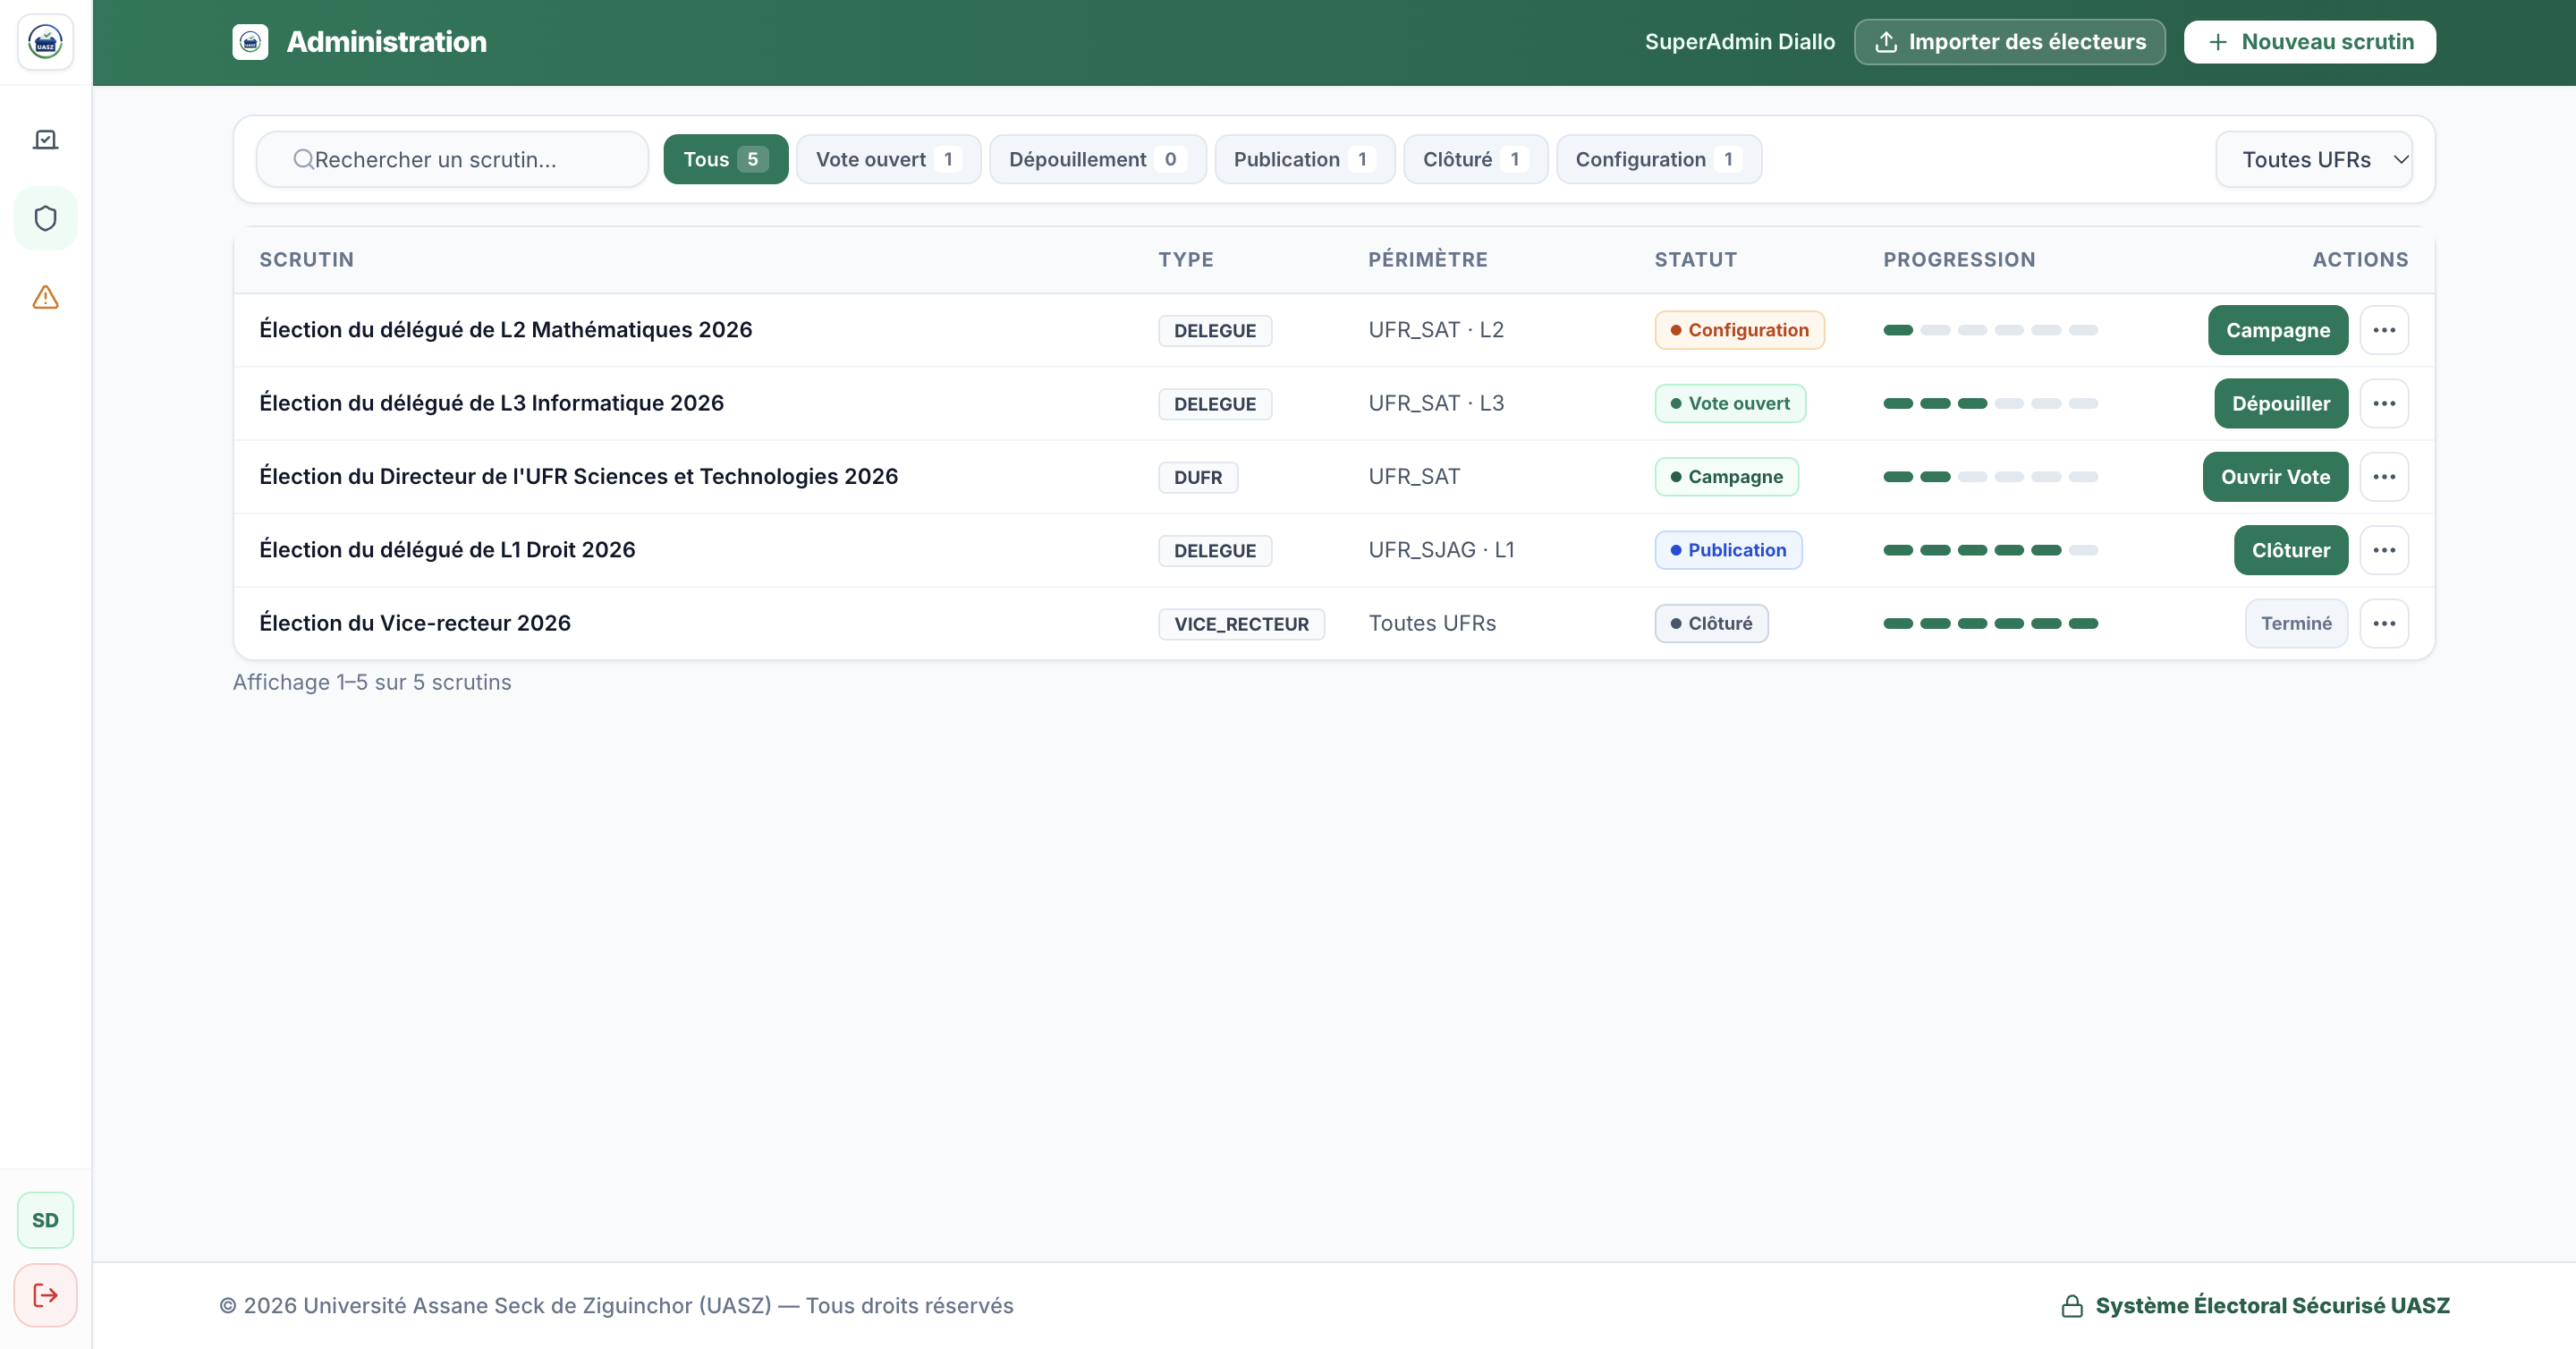
\includegraphics[width=0.92\textwidth,height=0.44\textheight,keepaspectratio]{3-2-5-admin-scrutins.png}
    \caption{Tableau de bord Super-Admin : gestion des scrutins (\texttt{/admin})}
    \label{fig:admin-scrutins}
\end{figure}

\begin{figure}[H]
    \centering
    \begin{minipage}{0.48\textwidth}
        \centering
        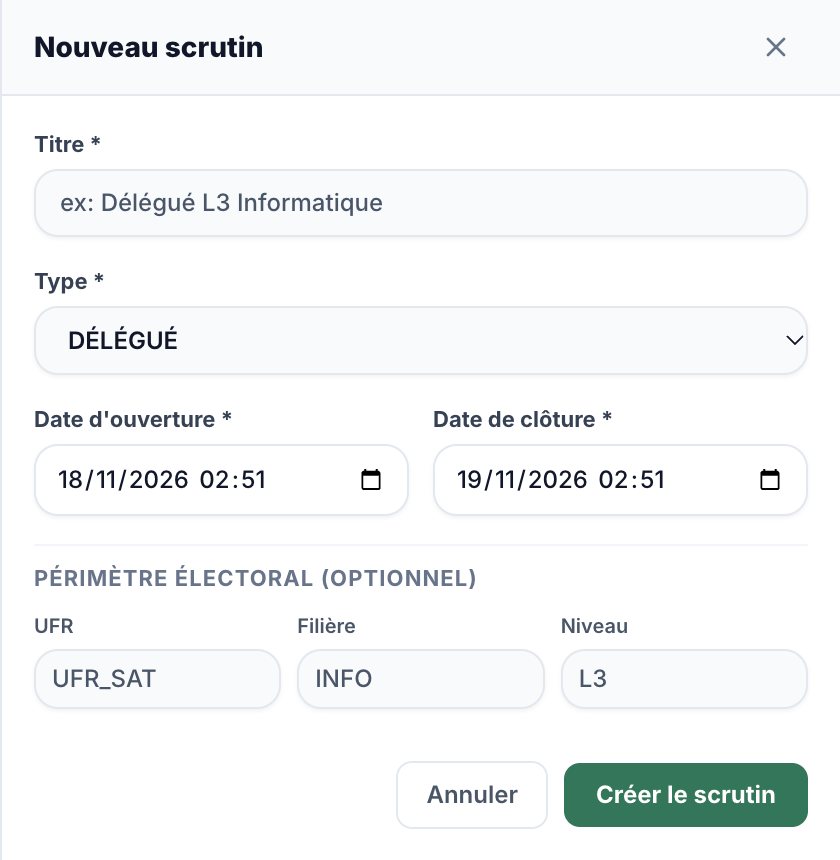
\includegraphics[width=\textwidth,height=0.38\textheight,keepaspectratio]{3-2-5-admin-nouveau-scrutin.png}
        \caption{Drawer de création d'un scrutin}
        \label{fig:admin-new}
    \end{minipage}
    \hfill
    \begin{minipage}{0.48\textwidth}
        \centering
        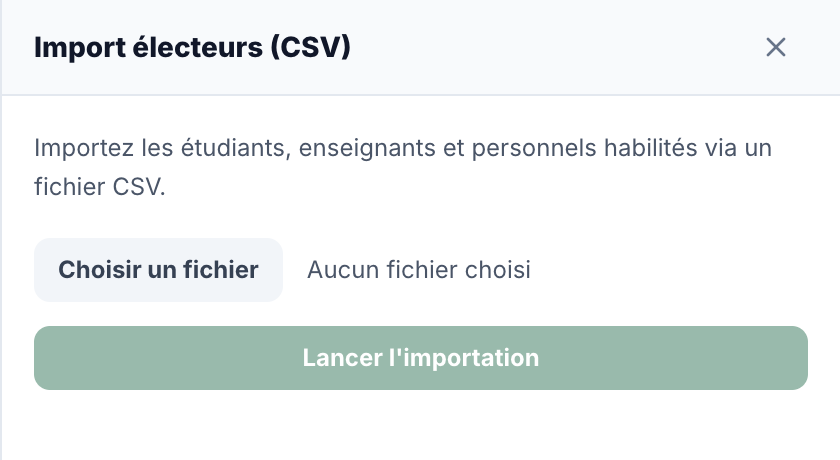
\includegraphics[width=\textwidth,height=0.38\textheight,keepaspectratio]{3-2-5-admin-import-csv.png}
        \caption{Import CSV des utilisateurs et résultat}
        \label{fig:admin-csv}
    \end{minipage}
\end{figure}

\begin{figure}[H]
    \centering
    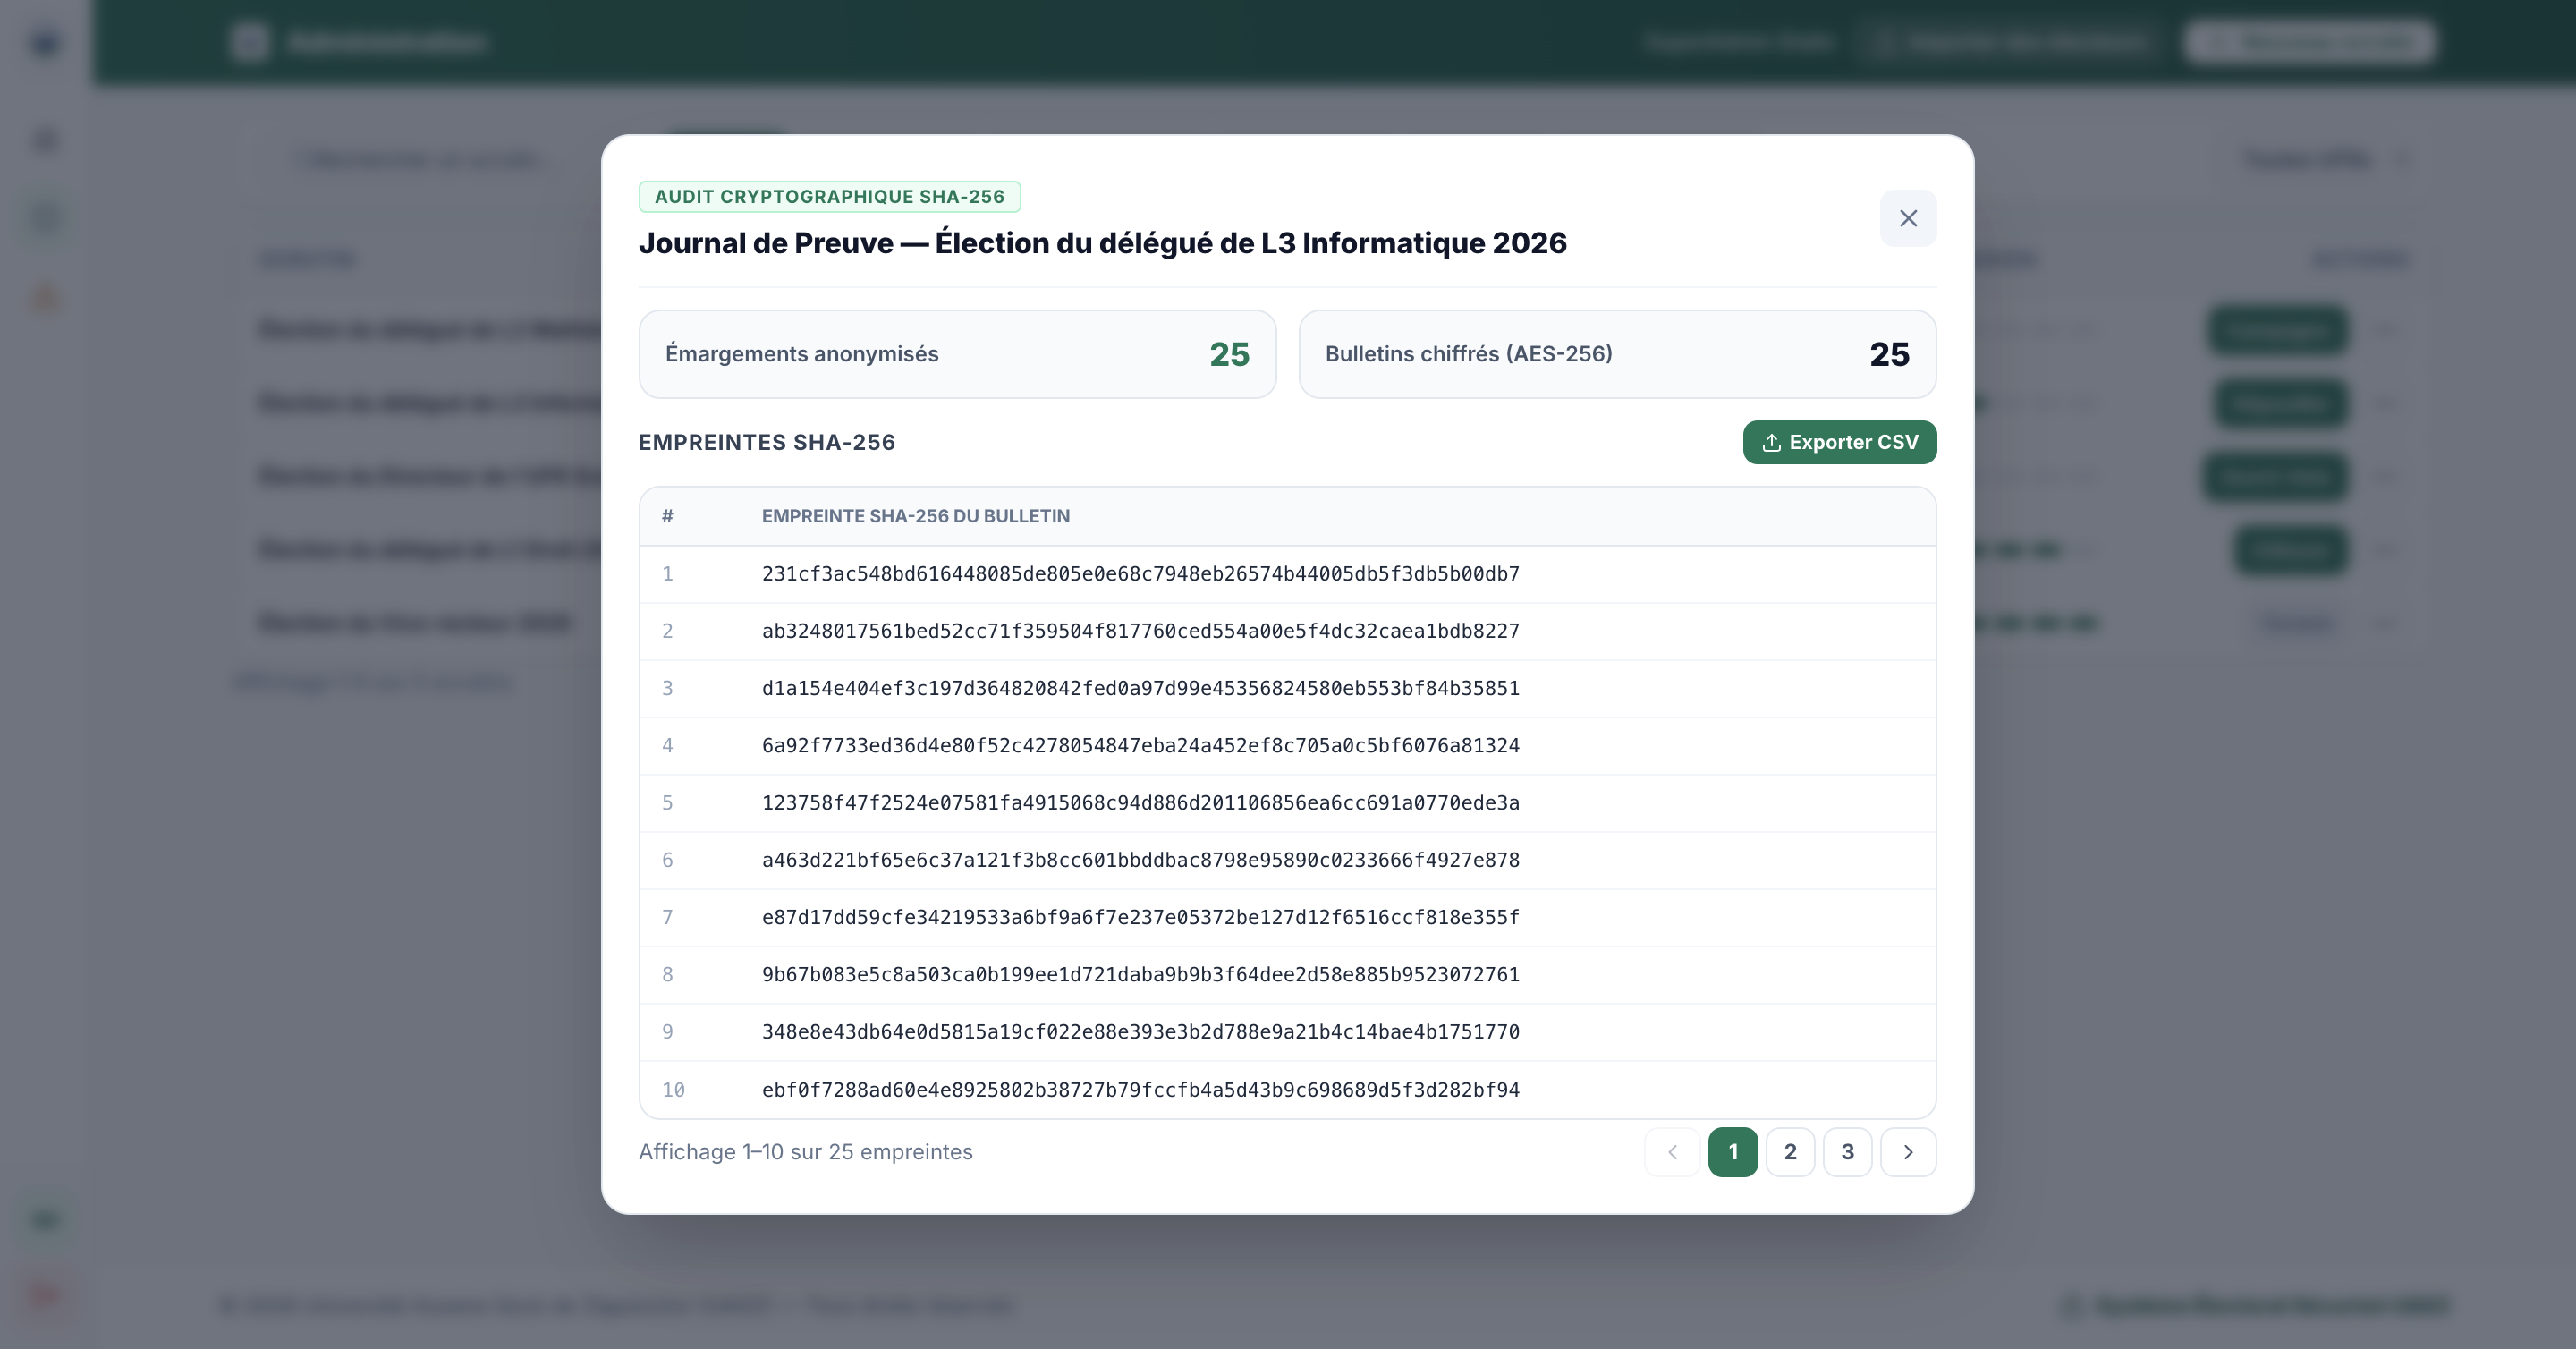
\includegraphics[width=0.92\textwidth,height=0.44\textheight,keepaspectratio]{3-2-5-admin-audit.png}
    \caption{Journal d'audit SHA-256 et export CSV (\texttt{/admin})}
    \label{fig:admin-audit}
\end{figure}

\begin{figure}[H]
    \centering
    \begin{minipage}{0.48\textwidth}
        \centering
        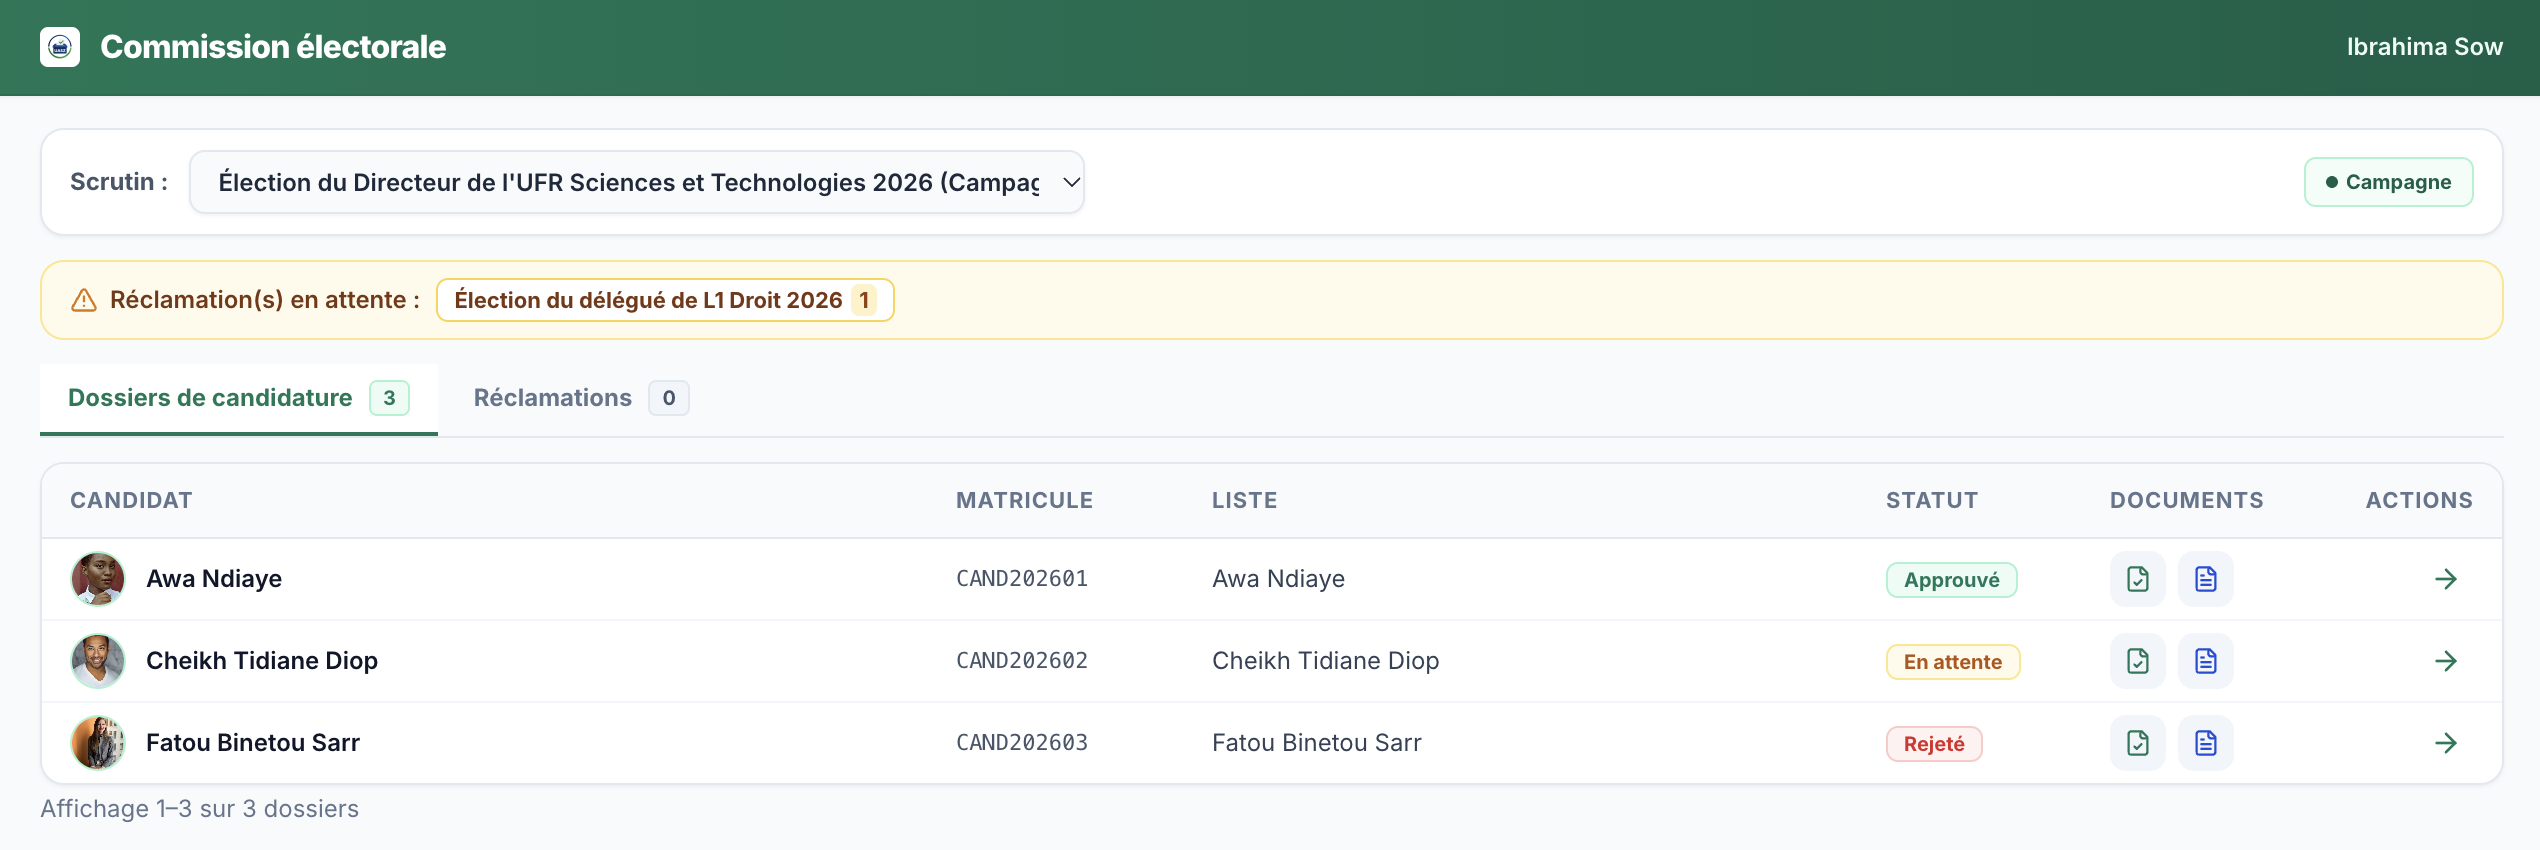
\includegraphics[width=\textwidth,height=0.38\textheight,keepaspectratio]{3-2-6-commission-dossiers.png}
        \caption{Commission : dossiers de candidatures}
        \label{fig:comm-dossiers}
    \end{minipage}
    \hfill
    \begin{minipage}{0.48\textwidth}
        \centering
        
\includegraphics[width=\textwidth,height=0.38\textheight,keepaspectratio]{3-2-6-commission-drawer.png}
        \caption{Drawer de validation / rejet motivé}
        \label{fig:comm-drawer}
    \end{minipage}
\end{figure}

\begin{figure}[H]
    \centering
    \begin{minipage}{0.48\textwidth}
        \centering
        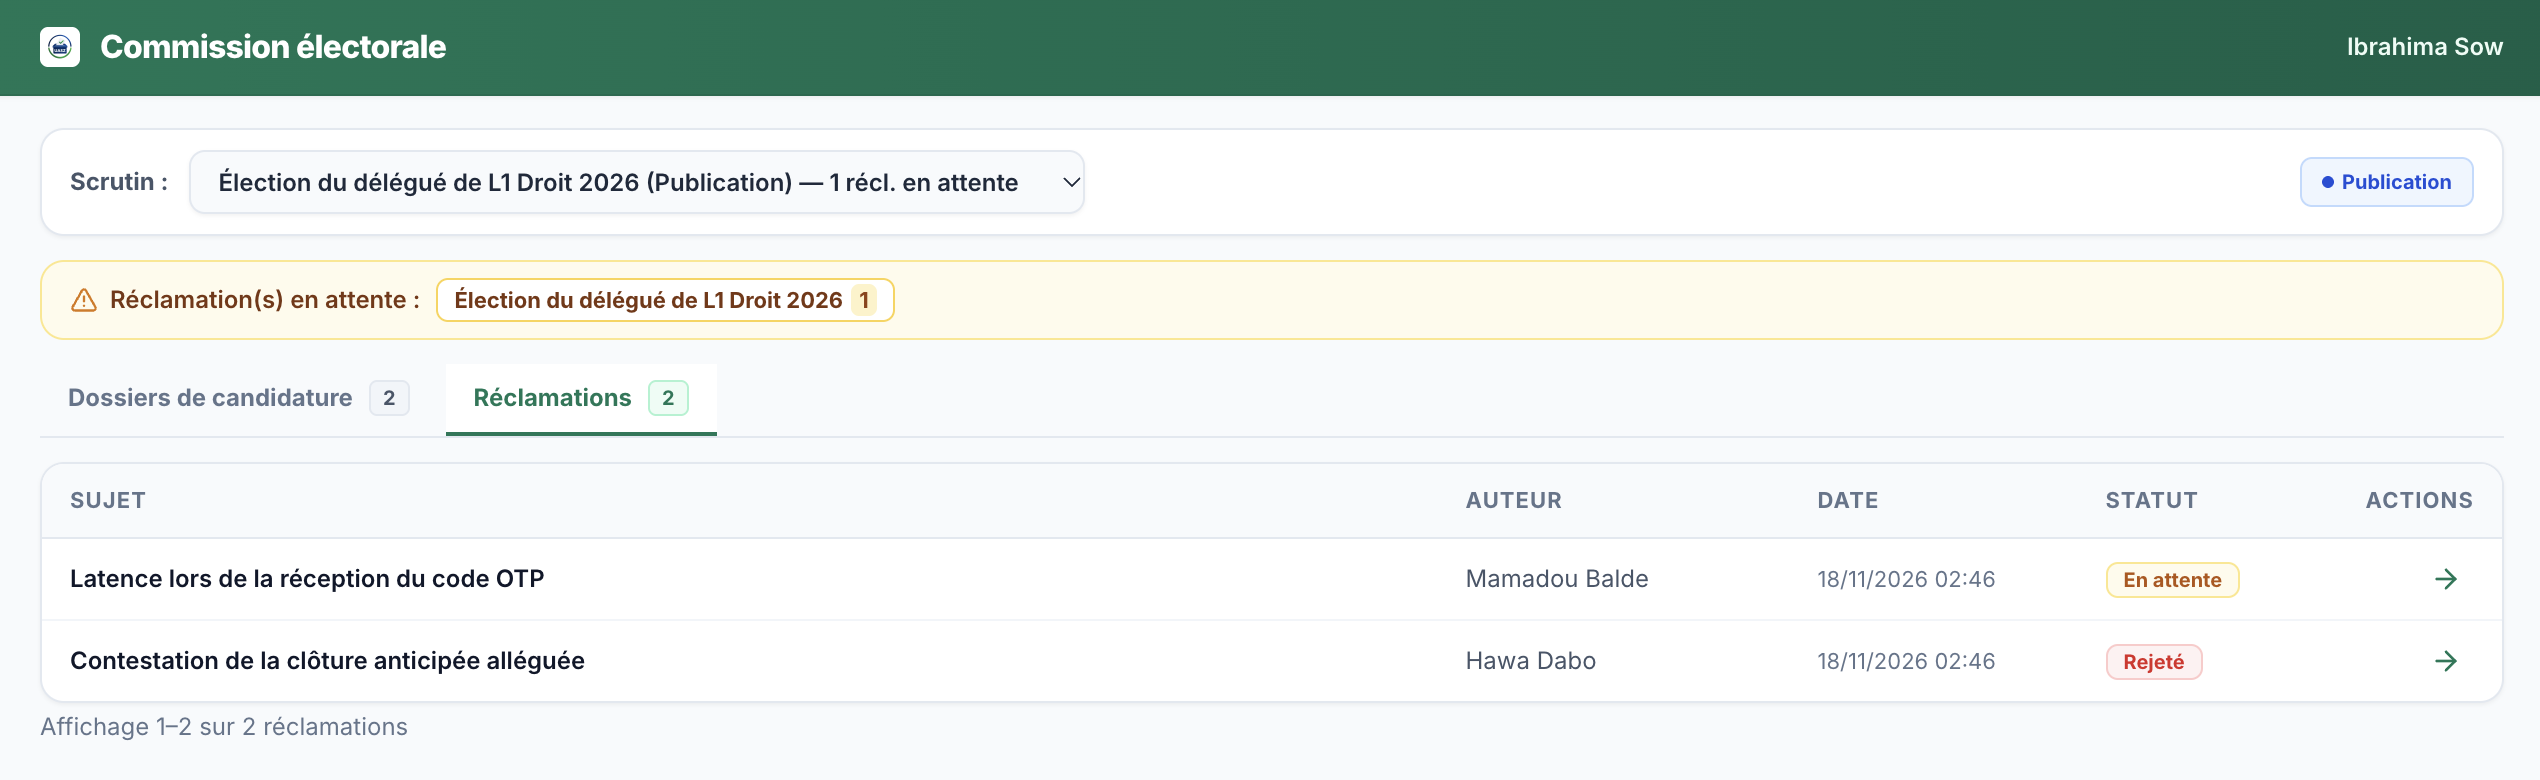
\includegraphics[width=\textwidth,height=0.38\textheight,keepaspectratio]{3-2-6-commission-reclamations.png}
        \caption{Traitement des réclamations (Commission)}
        \label{fig:comm-reclam}
    \end{minipage}
    \hfill
    \begin{minipage}{0.48\textwidth}
        \centering
        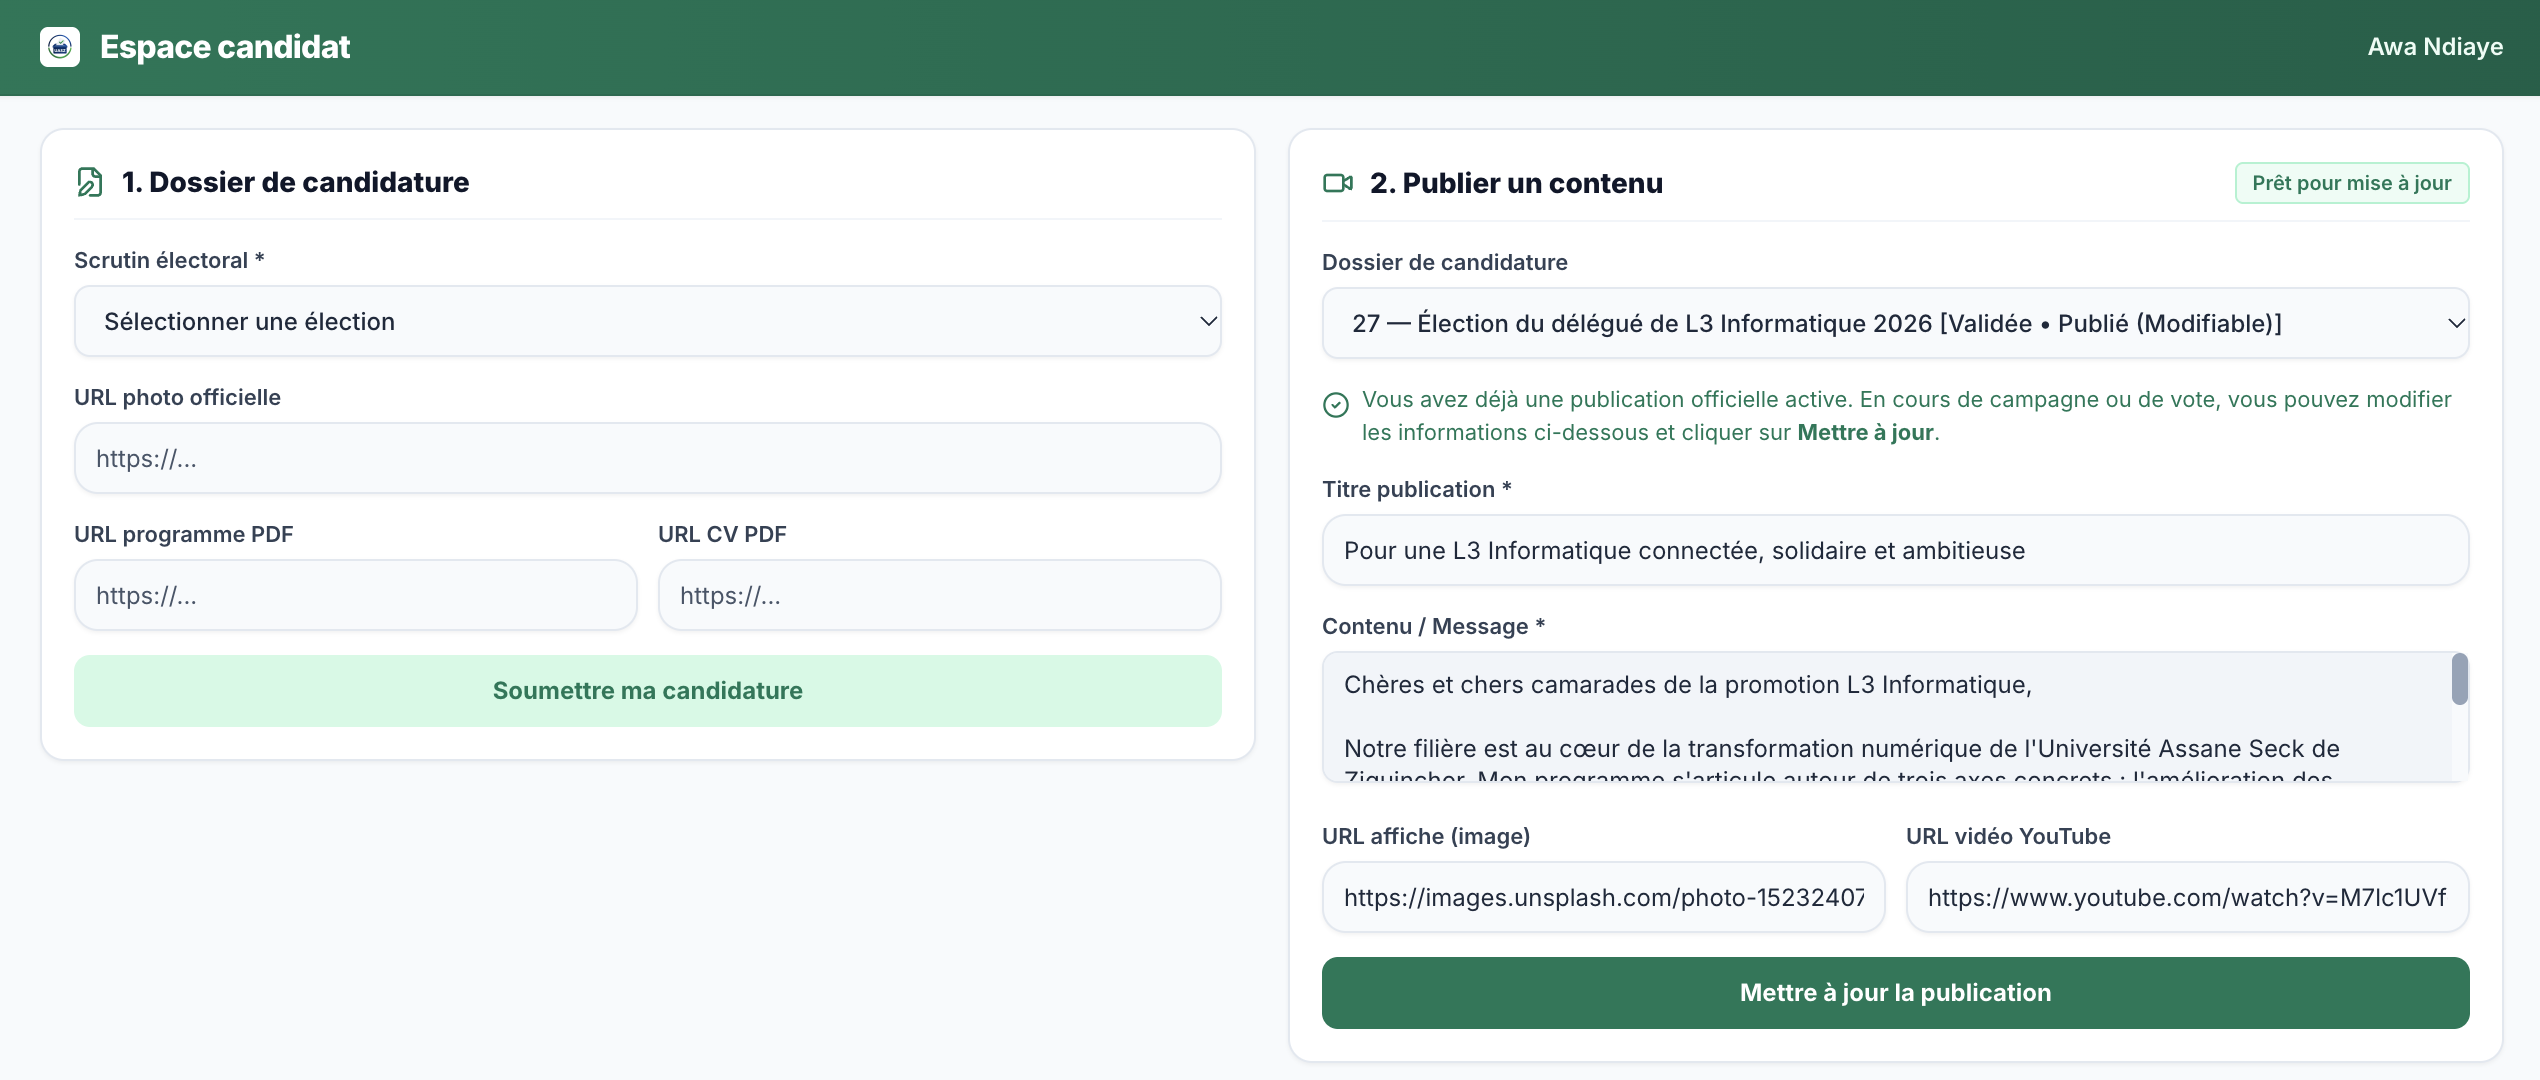
\includegraphics[width=\textwidth,height=0.38\textheight,keepaspectratio]{3-2-7-candidat-espace.png}
        \caption{Espace Candidat (\texttt{/candidat})}
        \label{fig:cand-espace}
    \end{minipage}
\end{figure}

\begin{figure}[H]
    \centering
    \begin{minipage}{0.62\textwidth}
        \centering
        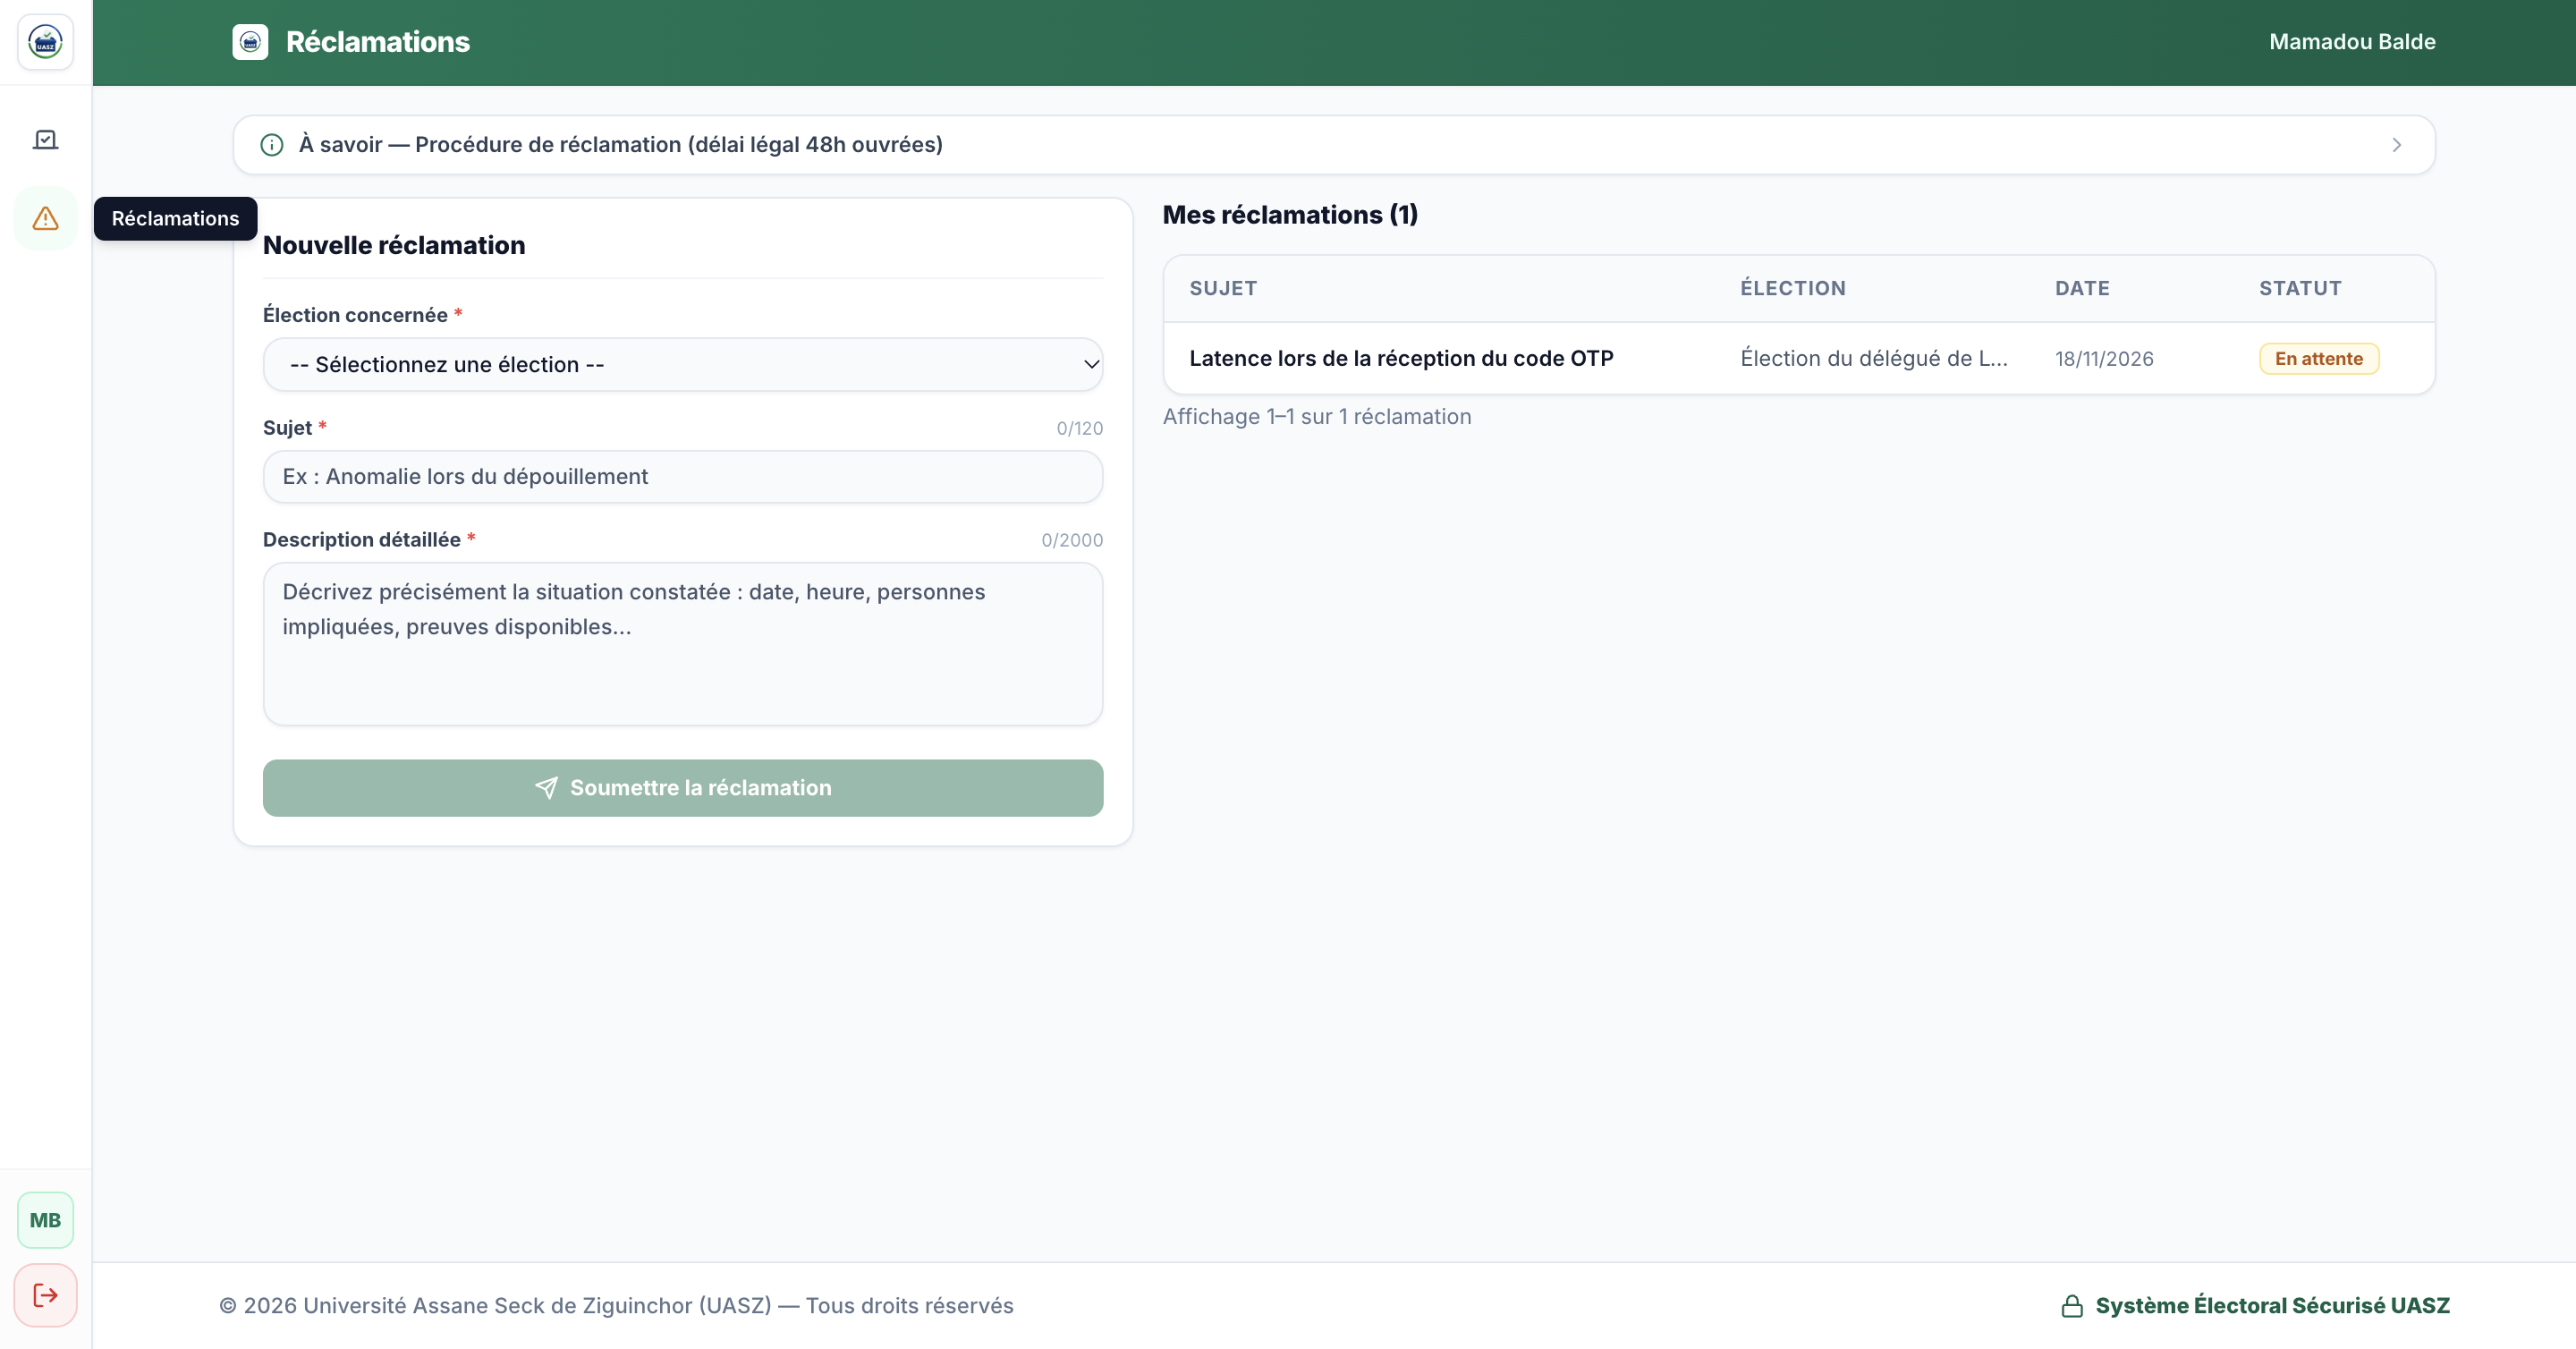
\includegraphics[width=\textwidth,height=0.40\textheight,keepaspectratio]{3-2-8-reclamations-electeur.png}
        \caption{Réclamations côté électeur (\texttt{/reclamations})}
        \label{fig:reclam-elec}
    \end{minipage}
    \hfill
    \begin{minipage}{0.34\textwidth}
        \centering
        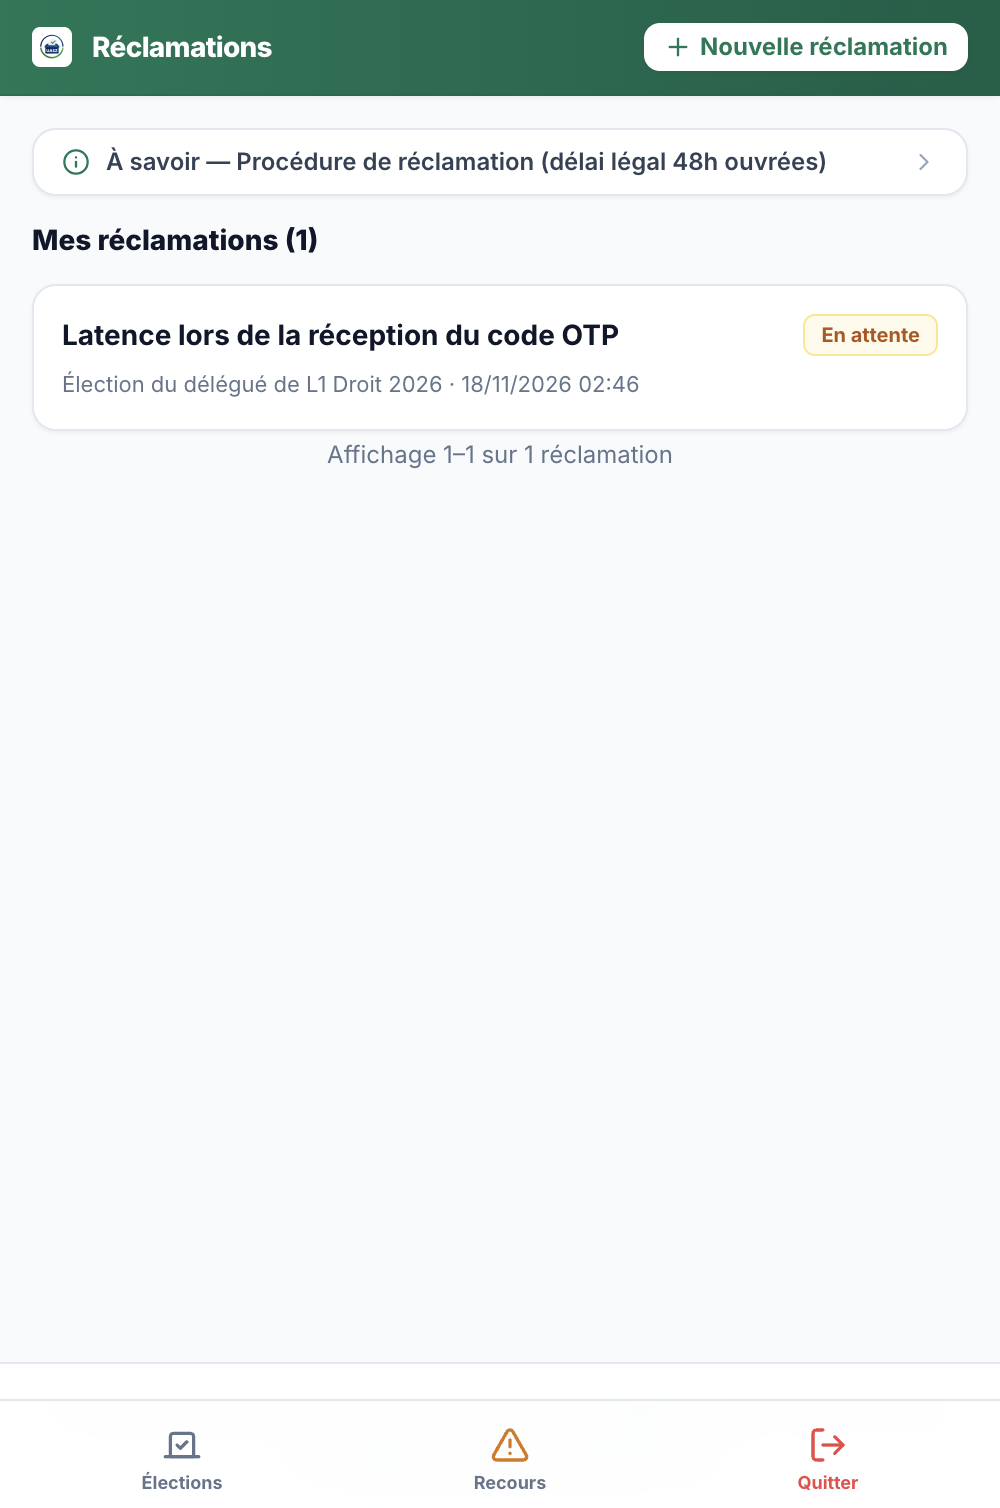
\includegraphics[width=\textwidth,height=0.40\textheight,keepaspectratio]{3-2-8-reclamations-mobile.png}
        \caption{Réclamations mobile (\texttt{390x844})}
        \label{fig:reclam-mob}
    \end{minipage}
\end{figure}

\begin{figure}[H]
    \centering
    \begin{minipage}{0.46\textwidth}
        \centering
        
\includegraphics[width=\textwidth,height=0.44\textheight,keepaspectratio]{3-2-9-pv-pdf.png}
        \caption{Procès-Verbal PDF généré (\textit{Vice-recteur 2026})}
        \label{fig:pv-pdf}
    \end{minipage}
    \hfill
    \begin{minipage}{0.50\textwidth}
        \centering
        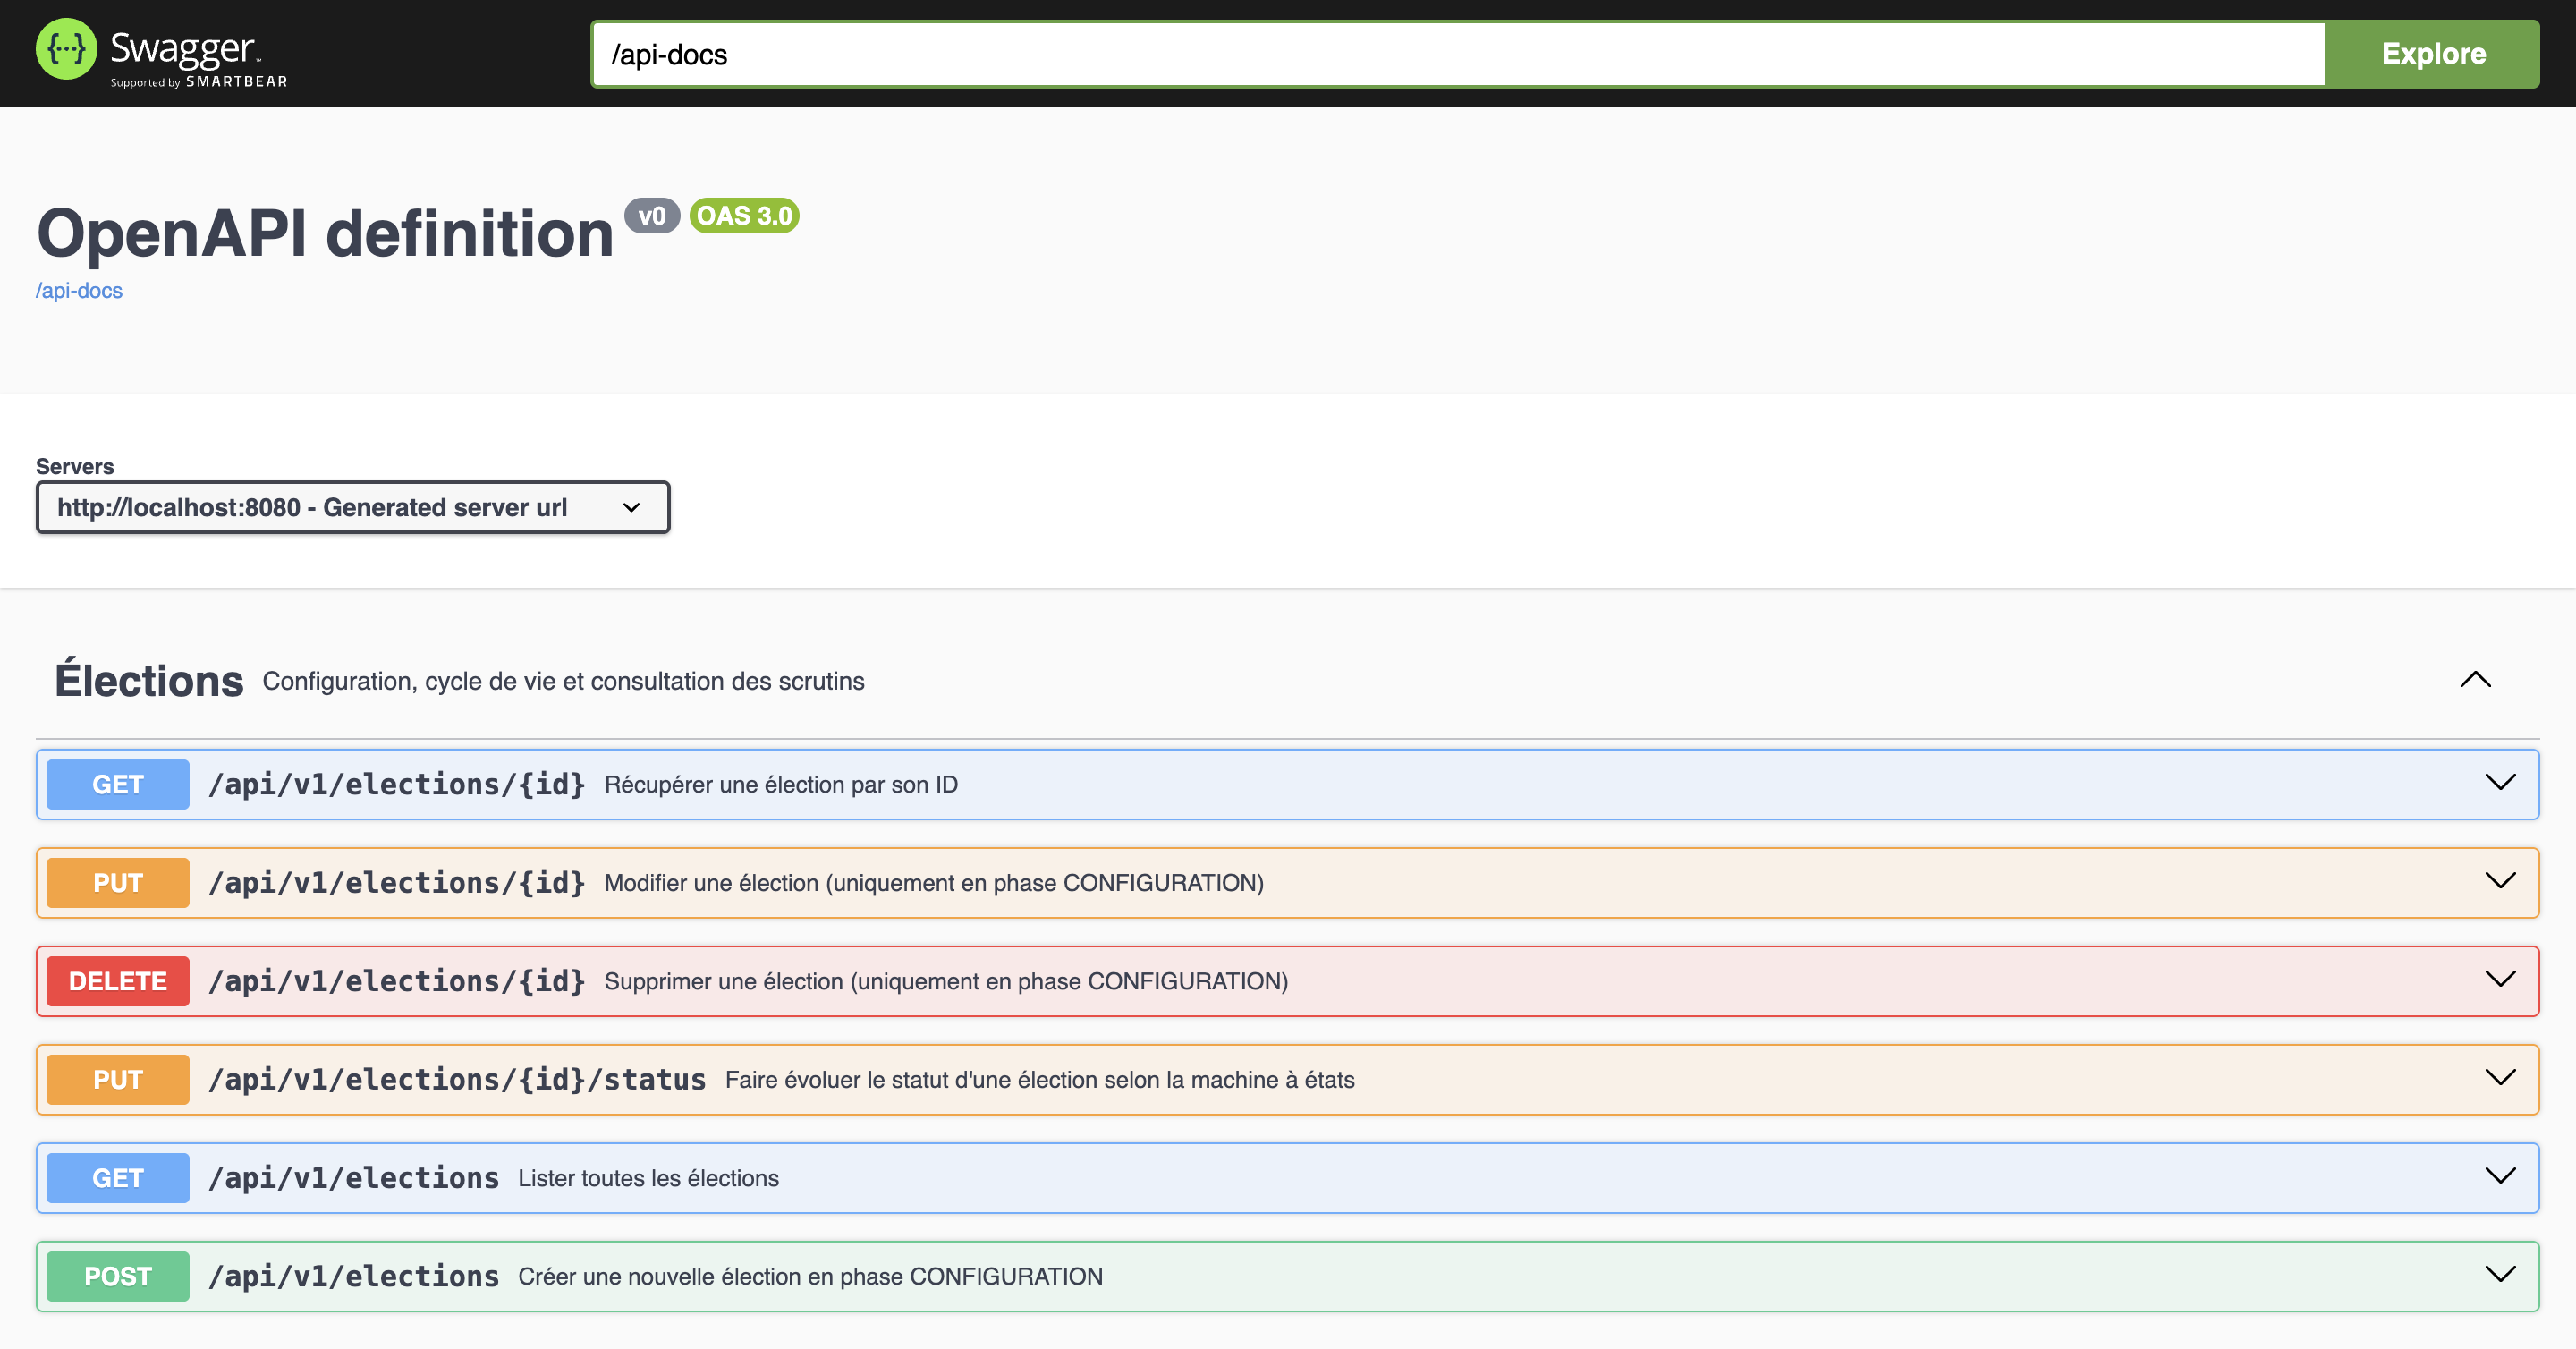
\includegraphics[width=\textwidth,height=0.44\textheight,keepaspectratio]{3-2-10-swagger-ui.png}
        \caption{Swagger UI (capture locale \texttt{localhost:8080})}
        \label{fig:swagger}
    \end{minipage}
\end{figure}

\section{Tests, qualité et critères de validation}

\subsection{Suite de tests Backend (\texttt{mvn -B verify})}
Exécutée sous Java 21, la commande \texttt{mvn -B verify} valide :
\begin{itemize}
    \item \textbf{Tests JUnit / Spring Boot} : \textbf{122 tests exécutés, 0 échec, 0 erreur, 0 ignoré} (\texttt{BUILD SUCCESS}).
    \item \textbf{Couverture JaCoCo 0.8.11 (50 classes)} : Instructions \textbf{74,30\,\%} (\texttt{5\,632/7\,580}), Branches \textbf{57,10\,\%} (\texttt{358/627}), Lignes \textbf{74,68\,\%} (\texttt{1\,233/1\,651}), Méthodes \textbf{70,39\,\%} (\texttt{164/233}), Classes \textbf{94,00\,\%} (\texttt{47/50}) (figure~\ref{fig:jacoco}).
    \item \textbf{Checkstyle 3.3.1} : \textbf{0 violation} (\texttt{backend/checkstyle.xml}).
\end{itemize}

\begin{figure}[H]
    \centering
    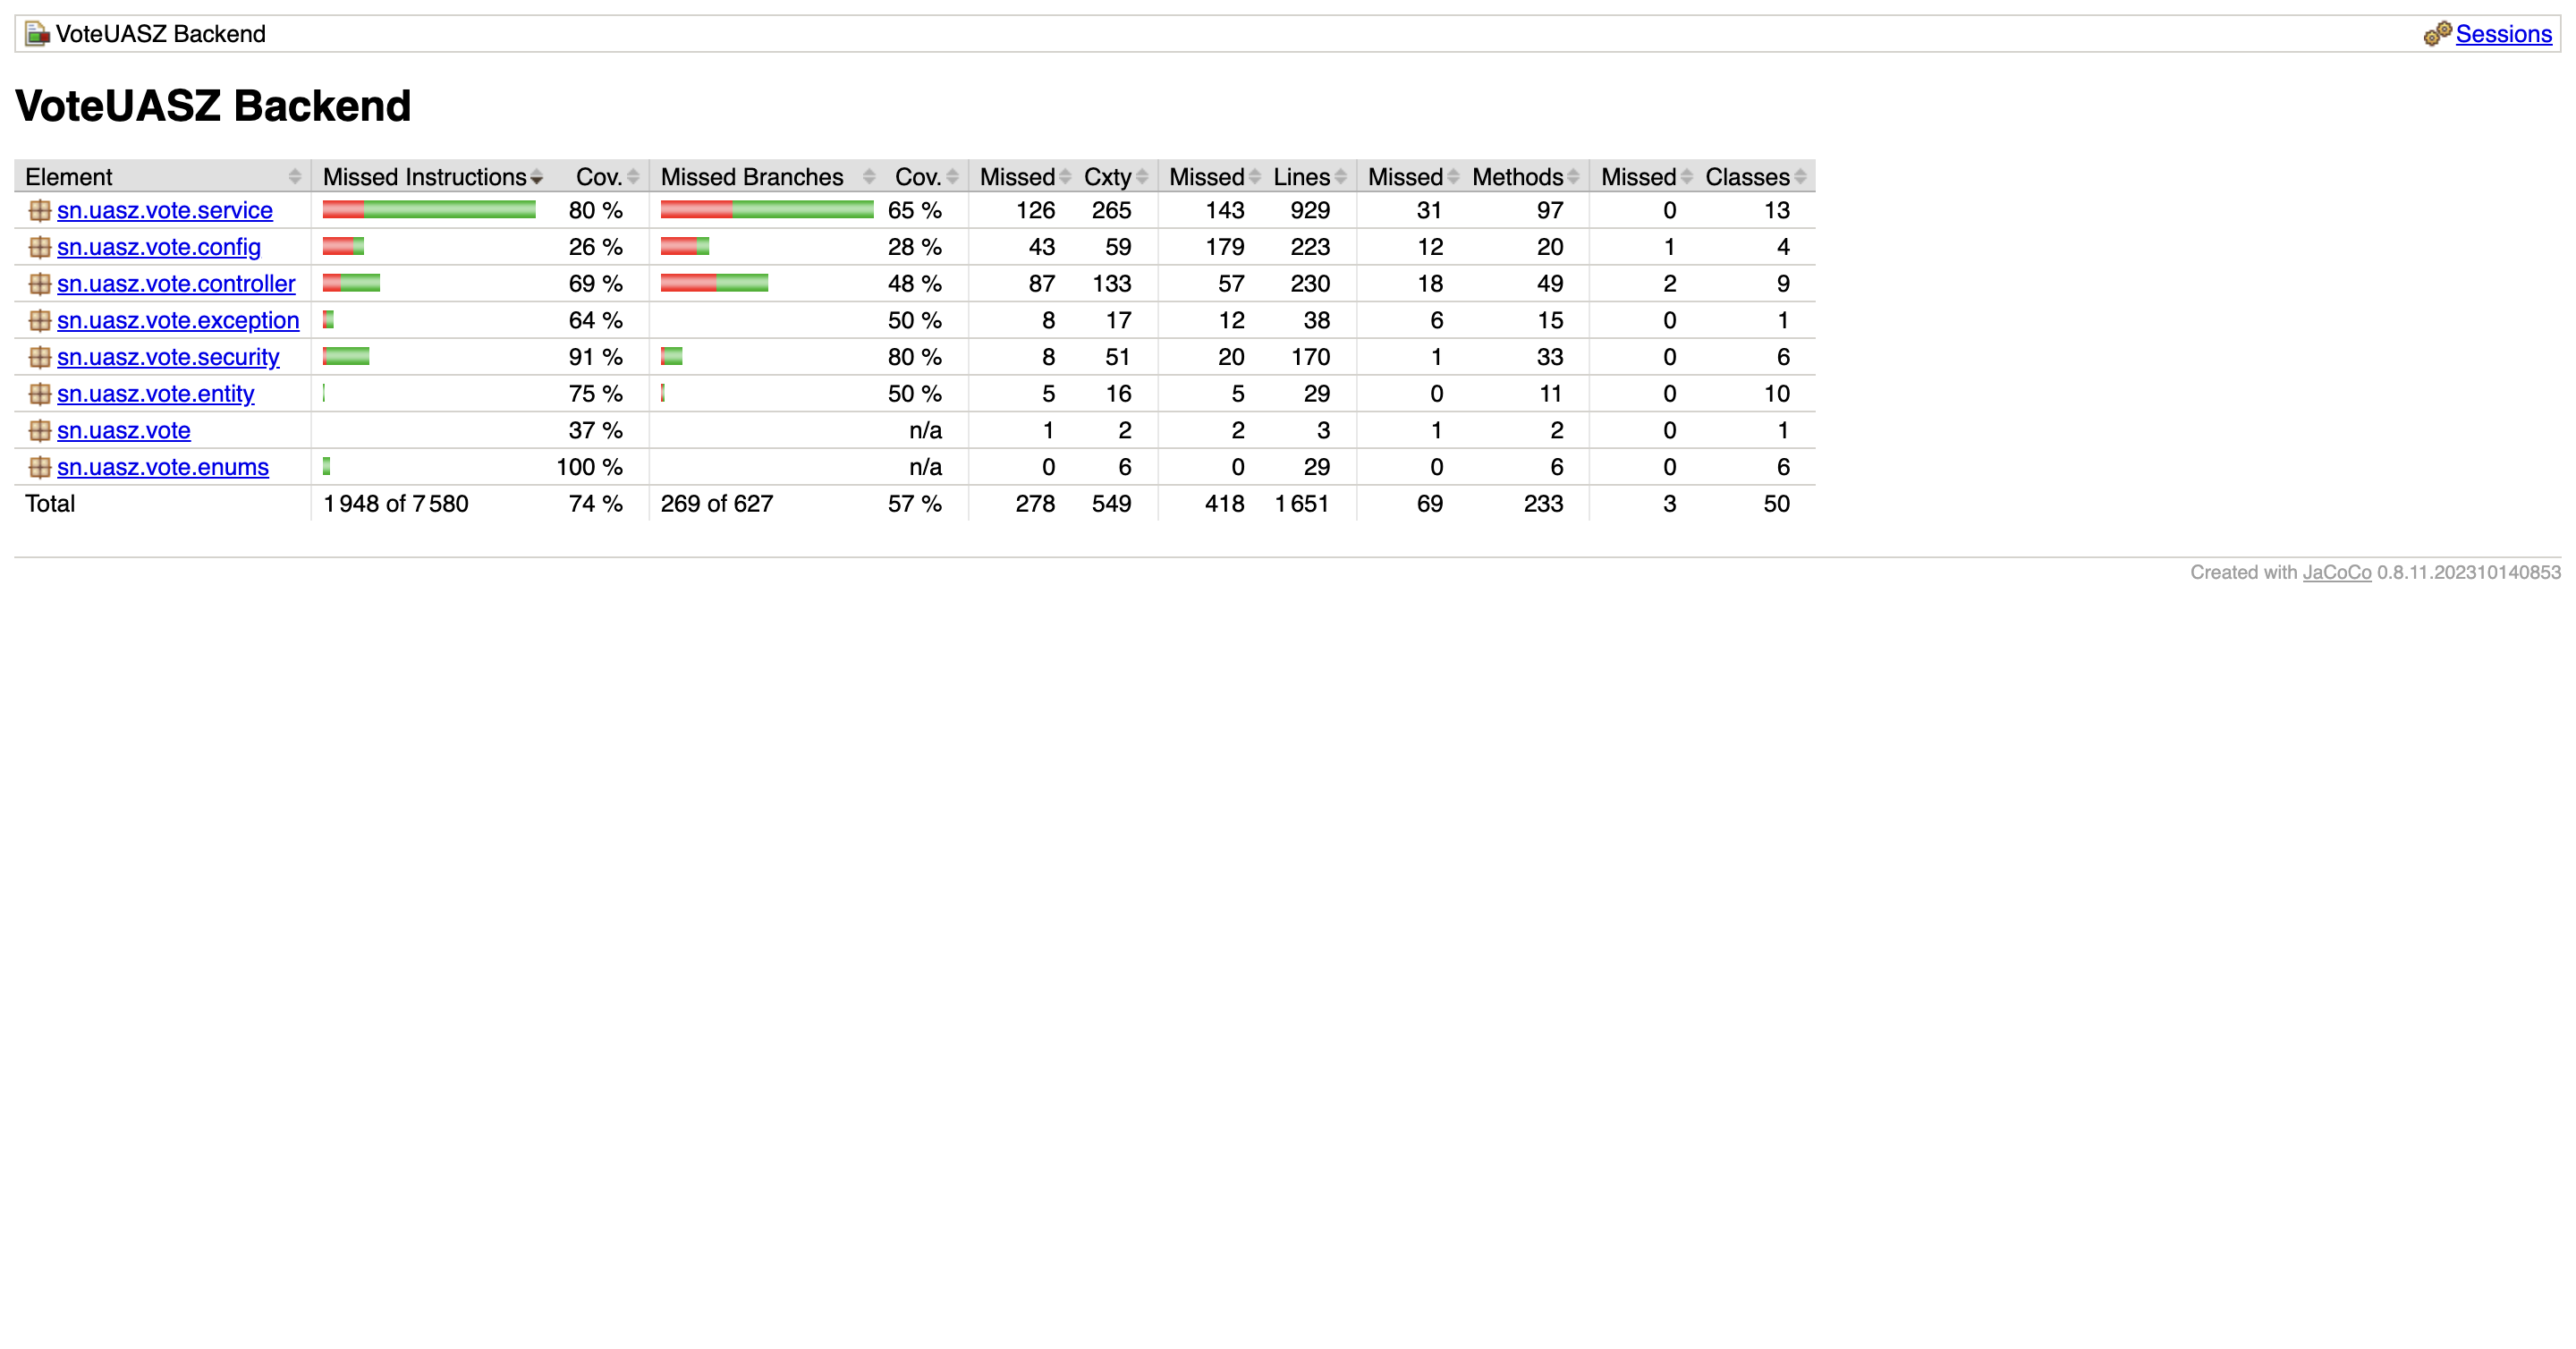
\includegraphics[width=0.92\textwidth,height=0.38\textheight,keepaspectratio]{4-1-jacoco.png}
    \caption{Rapport de couverture JaCoCo généré par \texttt{mvn -B verify}}
    \label{fig:jacoco}
\end{figure}

\subsection{Tests Frontend Angular et taille du bundle}
\begin{itemize}
    \item \textbf{Tests Karma/Jasmine (\texttt{ng test})} : \textbf{26 tests exécutés, 26 succès, 0 échec}.
    \item \textbf{Build de production (\texttt{ng build --configuration production})} : bundle initial total de \textbf{419,65\,kB} (\textbf{109,08\,kB} transférés) et \textbf{12 chunks} chargés à la demande.
\end{itemize}

\subsection{Synthèse des critères de validation}
\begin{table}[H]
\centering
\caption{Critères de validation : méthode et résultat réel mesuré}
\label{tab:criteres-validation}
\small
\begin{tabularx}{\textwidth}{@{}llX@{}}
\toprule
\rowcolor{uaszlight}
\textbf{Critère} & \textbf{Méthode} & \textbf{Résultat mesuré} \\
\midrule
Logique métier & \texttt{mvn -B verify} & \textbf{Réussi} : 122/122 tests, 74,30\,\% instructions, 0 violation Checkstyle. \\
Composants UI & \texttt{ng test} (ChromeHeadless) & \textbf{Réussi} : 26/26 tests passés. \\
Taille bundle & \texttt{ng build --configuration production} & \textbf{Réussi} : 419,65\,kB initial (109,08\,kB transférés). \\
Chaîne des bulletins & \texttt{AuditService.verifyBallotChain()} & \textbf{Réussi} : \texttt{chainValid=true} sur 25 + 3 + 4 bulletins réels. \\
Charge (\texttt{k6}) & Script \texttt{perf/load-test.js} & \textbf{Non testé} (\texttt{k6} non installé sur la machine locale). \\
Scan OWASP ZAP & \texttt{.github/workflows/zap-baseline.yml} & \textbf{Non testé} localement (workflow manuel GitHub Actions). \\
Performance 3G & Lighthouse avec throttling 3G & \textbf{Non testé} (à exécuter sur l'environnement de production). \\
\bottomrule
\end{tabularx}
\end{table}

\section{Déploiement Cloud}

Le déploiement continu s'appuie sur \texttt{render.yaml} (service Docker Java 21 + base PostgreSQL 16 \texttt{voteuasz-db} sur Render, avec variables \texttt{JWT\_SECRET}, \texttt{CRYPTO\_SECRET}, \texttt{AUDIT\_IP\_SALT} et \texttt{BREVO\_API\_KEY}) et \texttt{vercel.json} (build Angular 17 et réécriture \texttt{/api/(.*)} vers le backend Render). L'environnement local est orchestré via \texttt{docker-compose.yml} (PostgreSQL 16 sur port 5540 et MailHog sur ports 1025/8025).

\section{Synthèse vs cahier des charges, écarts justifiés et limites}

\begin{table}[H]
\centering
\caption{Écarts justifiés entre le cahier des charges initial et le code réel}
\label{tab:ecarts}
\small
\begin{tabularx}{\textwidth}{@{}lXX@{}}
\toprule
\rowcolor{uaszlight}
\textbf{Fonction prévue} & \textbf{Implémentation réelle} & \textbf{Justification} \\
\midrule
OTP par SMS & OTP par e-mail (Brevo HTTPS API / SMTP) & Absence de passerelle SMS payante ; l'e-mail institutionnel reste gratuit et traçable. \\
Export PV JasperReports & Génération programmatique via OpenPDF 1.3.30 & Poids réduit, aucune dépendance à un moteur \texttt{.jrxml} externe. \\
Upload binaire médias & URLs externes (\texttt{photoUrl}, \texttt{programmePdf}, \texttt{cvUrl}, \texttt{afficheUrl}) & Système de fichiers éphémère sur Render Free sans stockage objet S3/Cloudinary. \\
Tests CI Testcontainers & Base H2 en mémoire (\texttt{@Profile("test")}) & Exécution rapide sans démon Docker requis en CI. \\
Mode hors-ligne complet & PWA Angular (\texttt{ngsw-config.json}) pour les assets & Le dépôt de vote nécessite une validation OTP et transactionnelle en ligne. \\
\bottomrule
\end{tabularx}
\end{table}
